\documentclass[12pt,a4paper]{article}
\usepackage[utf8]{inputenc}
\usepackage[czech, english]{babel}
\usepackage[T1]{fontenc}
\usepackage{amsmath}
\usepackage{amsfonts}
\usepackage{amssymb}
\usepackage{graphicx}
\usepackage[final,pdftex, colorlinks=false]{hyperref}
\usepackage{xcolor}

\usepackage{multirow}
\usepackage{graphicx}
\usepackage{booktabs}

\newcommand{\mcrot}[4]{\multicolumn{#1}{#2}{\rlap{\rotatebox{#3}{#4}~}}} 
\newcommand*{\twoelementtable}[3][l]%

%\usepackage{comment}
%\usepackage{floatrow}
%\usepackage{multirow}
%\usepackage{algorithm}
%\usepackage{algorithmicx}
%\usepackage{algpseudocode}
%\usepackage{titletoc}
%\usepackage{pdfpages}
%\usepackage{hhline}
%\usepackage{makecell}

\usepackage{listings}			%vkladani kodu
\lstset{basicstyle=\ttfamily,
  showstringspaces=false,
  commentstyle=\color{red},
  keywordstyle=\color{blue},
  breaklines=true,
  frame=lines,
}

%okraje
\usepackage[
left=35mm,
right=25mm,
top=40mm,
bottom=35mm]
{geometry}

\author{David Těthal}

%%%%%%%%%%Prikazy%%%%%%%%%%
\renewcommand\baselinestretch{1.3}		%radkovani
\parskip=0.8ex plus 0.4ex minus 0.1 ex	%mezera mezi odstavci

\newcommand{\keywords}[2]{\noindent\textbf{#1: }#2}
\newcommand{\necislovana}[1]{%
\phantomsection
\addcontentsline{toc}{section}{#1}

%\newcommand{\exedout}{%
%  \rule{0.8\textwidth}{0.5\textwidth}%
%}


\section*{#1}
\markboth{\uppercase{#1}}{}
}
%%%%%%%%%%%%%%%%%%%%%%%%%%%%

%%%%%%%%%%Zahlavi%%%%%%%%%%%
\usepackage{fancyhdr}
\fancyhead[L]{ČVUT v Praze}
\setlength{\headheight}{16pt}
%%%%%%%%%%%%%%%%%%%%%%%%%%%%

\begin{document}
\pagestyle{empty}

%titulni strana
\newpage
\begin{center}
%napisy
\newcommand{\napisCVUT}{České vysoké učení technické v Praze}
\newcommand{\napisFS}{Fakulta Stavební}
\newcommand{\napisProgram}{Studijní program Geodézie a Kartografie}
\newcommand{\napisObor}{Obor Geomatika}
\newcommand{\napisKatedra}{Katedra Geomatiky}
\newcommand{\napisVedouci}{Vedoucí: Ing. Martin Landa, Ph.D.}
\newcommand{\napisAutor}{Bc. David Těthal}
\newcommand{\napisDatum}{Praha 2018}
\newcommand{\napisNazevI}{Rozšíření platformy Gisquick o podporu časoprostorových dat}
\newcommand{\napisDiplomka}{Diplomová práce}
%
% prikazy
%\newcommand{\velka}[1]{\uppercase{#1}}
\newcommand{\velka}[1]{\textsc{#1}}
%
% 
\newif\ifpatitul
\patitultrue


{\Large\velka{\napisCVUT}}\\
{\Large\velka{\napisFS}}\\
{\Large\velka{\napisProgram}}\\
{\Large\velka{\napisObor}}
\vfill

\includegraphics[width=3cm]{./img/logo_cvut_cb} %~
\vfill
{\Large\velka{\napisDiplomka}}\\
\Large\velka{\napisNazevI}\\
\vfill
{\large%
\napisVedouci\\
\napisKatedra\\
\bigskip
\napisDatum\hfill\napisAutor}
\end{center}


%zadani prace
\newgeometry{left=1.8cm,top=2cm} 
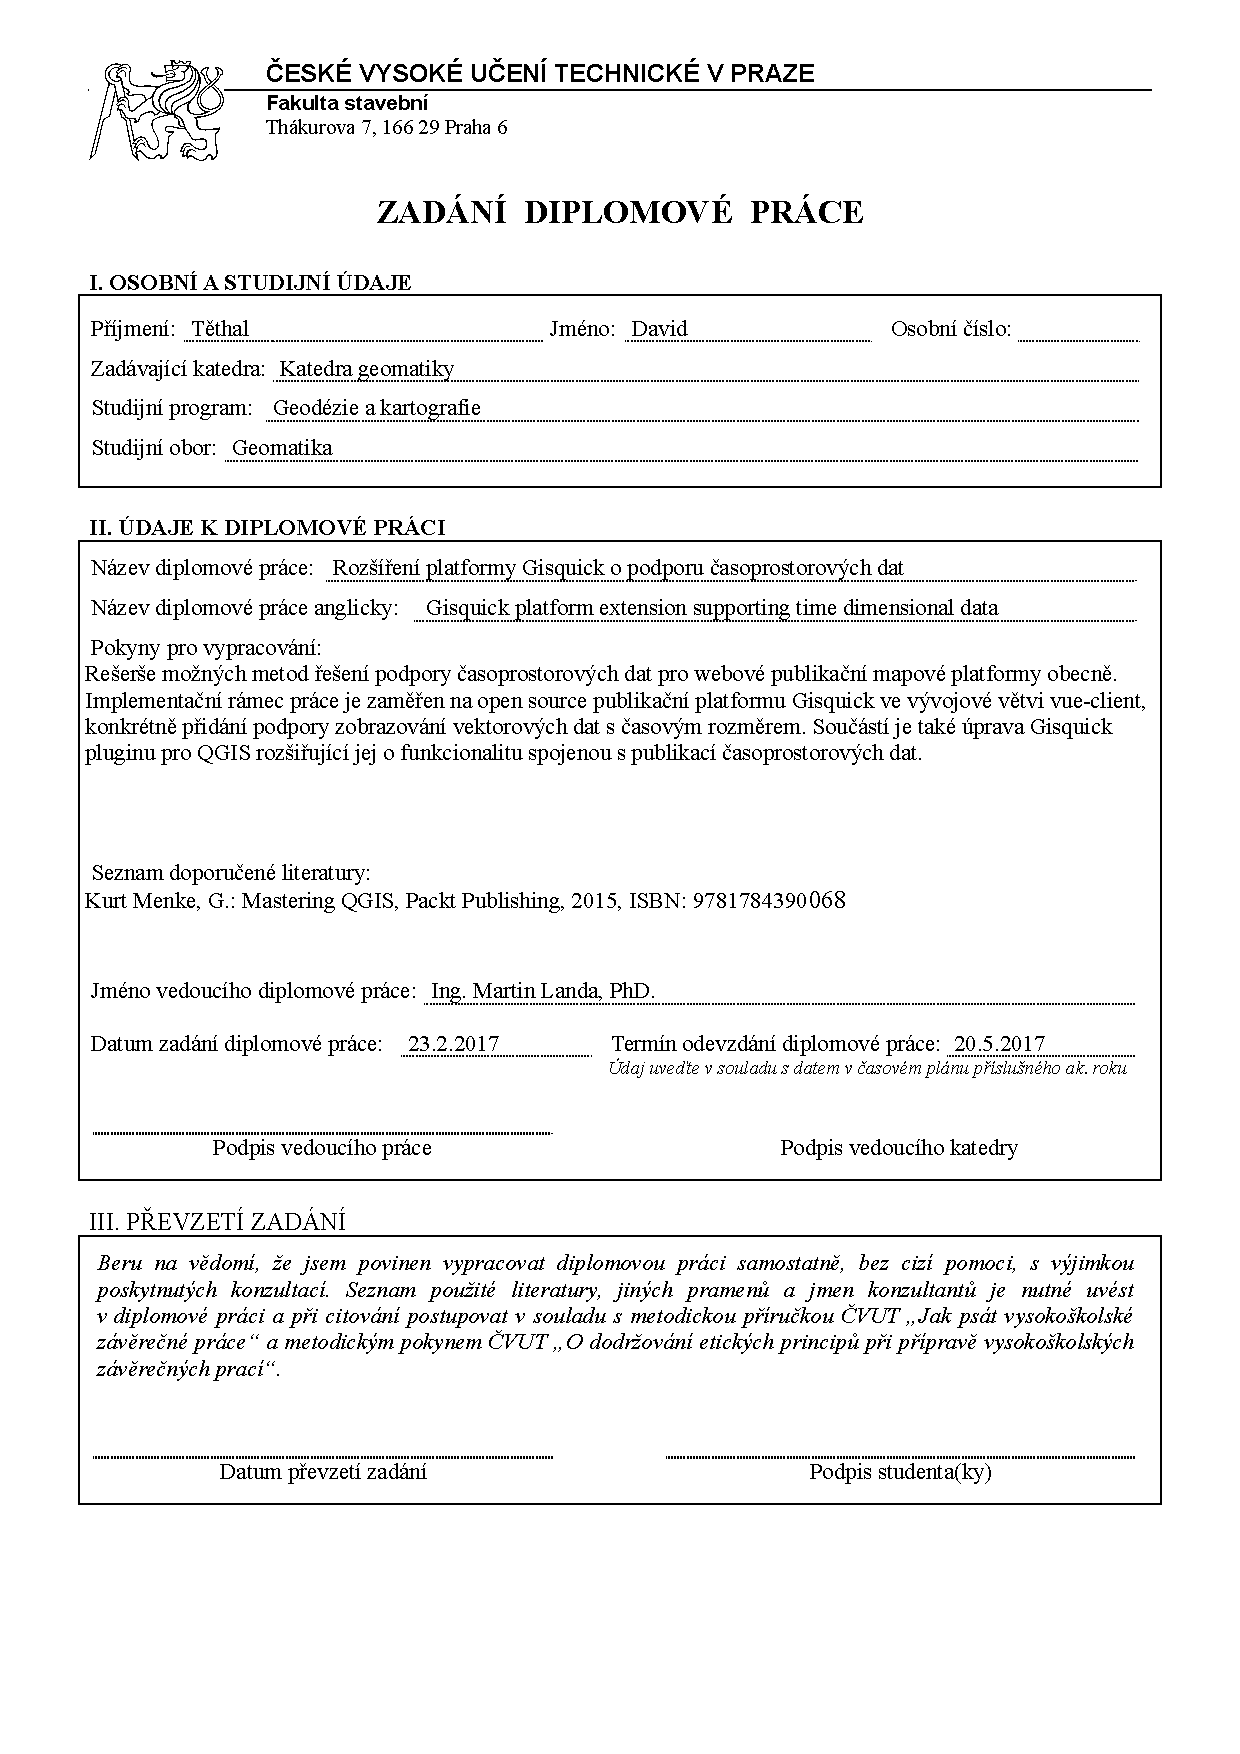
\includegraphics[scale=0.8]{../zadani/zadanidp}
\restoregeometry

%abstract CS
\newpage
\selectlanguage{czech}
\begin{abstract}
\bigskip
Cílem této diplomové práce je navrhnutí a vytvoření nástroje rozšiřujícího platformu Gisquick o podporu práce s časoprostorovými daty. Nástroj nabídne uživateli přehledné uživatelské rozhraní, které umožní možnost filtrace vektorových vrstev na základě jejich časových dat. Nad daty bude rovněž možnost tvorby jednoduché animace dle vybraného časového kroku.

Práce dále zahrnuje rešerši fungování webových publikačních platforem a nastínění jejich metod řešení pro práci s časoprostorovými daty. Na základě rešerše byla zvolena optimální metoda, která byla posléze vhodně aplikované na již stávající platformu.

Další část práce se zabývá implementací nalezeného řešení na straně Gisquick klienta. Nástroj byl vyvíjen v programovacím jazyce JavaScript s použitím frameworku Vue.js, do kterého je v tuto chvíli webový klient přepisován. Spolu s úpravy klienta bylo dále nutné zahrnout novou funkcionalitu do zásuvného modulu Gisquick plugin pro QGIS, sloužícího k publikaci předem vytvořených projektů. V pluginu je možné jednotlivé vrstvy před publikací nastavit a identifikovat jejich atribut obsahující časovou složku.

\bigskip
\bigskip
\keywords{Klíčová slova}
OGC WMS, časoprostorová data, QGIS, JavaScript, Python, Vue.js, plugin.
\end{abstract}


%Absktrakt anglicky
\newpage
\selectlanguage{english}
\begin{abstract}
	\bigskip
Main goal of my thesis was design and implementation of new tool into Gisquick platform, that is focused on handling with spatio-temporal data. Gisquick platform provides fast and easy QGIS project publication. New tool will enable users to work easily with layers containing time attribute, filter its content and make simple animations.

First part was focused on web map platforms. This chapter contains brief description of procces that produce requested map for user. Second part of the first chapter describes existing solutions for spatio-temporal data handling that may be used for web map platforms in general. 
	
	\bigskip
	\bigskip
	\keywords{Klíčová slova}
	klicova slova
\end{abstract}


%Prohlaseni a podekovani
\selectlanguage{czech}
\newcommand{\odsaditodzhora}{\hskip1pt\vfill}
\newpage
\odsaditodzhora
\noindent {\bf Prohlášení}
Tímto prohlašuji, že diplomovou práci na uvedené téma jsem včetně výzkumu a implementace vypracoval samostatně.
Použitá literatura a podkladové materiály jsou uvedeny v seznamu zdrojů.


\begin{flushleft}
\begin{tabular}{cp{0.3\textwidth}c}
V Praze .................
& 
&
..................................
\\
&&
(podpis autora)
\end{tabular}

\end{flushleft}
\newpage

\odsaditodzhora
\noindent {\bf Poděkování}
text poděkování
\newpage
\tableofcontents

\newpage
\pagestyle{fancy}

\necislovana{Úvod}

Časoprostorová data jsou pro mnoho lidí velice obecný pojem, pod
kterým si často nedovedou nic konkrétního představit. Takto označovaná
data jsou v dnešní době již běžně používána ve velké řadě oborů od
archeologie, geodézie, geologie, stavebního inženýrství, územního
plánování až po armádní účely, zemědělství a meterologii. Nejedná se
tedy v žádném případě o specializovaný termín používaný pouze v jednom
vědním oboru.

%% ML: Na jedne strane?
Práci s časoprostorovými daty lze rozdělit na dvě skupiny. Na jedné
jsou odborníci, kteří časoprostorová data sbírají, provádějí analýzy,
vyhodnocují je pomoci specializovaných programů a vytvářejí nad nimi
tématické mapy. Na druhé straně je poté široká veřejnost, která
používá pouze finální produkt jejich práce.

V dřívější době byla možnost publikace těchto dat jen velice
omezena. To se v dnešní době s rozšířením internetu a nástupem
elektronicky publikovaných map pomoci publikačních platforem rapidně
%% ML: male p anebo do uvozovek
změnilo. Právě Publikační platformy vyplňují mezeru mezi odborníky a
širokou veřejností, kdy dávají téměř každému možnost prezentace dat v
ucelené formě.


Spojení publikační platformy a časoprostorových dat je potom dalším
krokem, který možnost prezentace dat ještě umocní. Pomocí vhodně
vytvořených nástrojů pro filtrování dat na základě jejich časové osy
se dají vytvářet simulace zobrazující průběh určitého vlivu v čase na
určitém místě. Tímto způsobem se dá například jednoduchým způsobem
simulovat vývoj požárů, migrace zvěře, nebo expanze měst. Pro
uživatele lepšího časového vjemu lze rovněž dosáhnout, vytvořením
názorné animace, kdy se zobrazovaný stav mění s předem nastaveným
časovým krokem.

Jednou z takových publikačních platforem je právě Gisquick. V tomto
případě se navíc jedná o interaktivní platformu, kde může uživatel
nejenom na data nahlížet, ale také měnit způsob jejich vizualizace. Ke
stávajícím datům se rovněž dají přidat podkladové vrstvy, které
uživateli zlepší celkový pohled na zobrazovanou situaci. Výhodou při
publikaci časoprostorových dat na platformě Gisquick je také jejich
univerzálnost. Nezáleží tedy, zdali jsou data s odstupem minut či
roků. Díky jednoduchému nastavení lze nástroj přizpůsobit téměř
jakémukoli časovému intervalu. Velká benevolence je rovněž ve vstupním
formátu časového řetězce.

\bigskip
Na platformu Gisquick resp. její rozšíření o podporu pro
časoprostorová data se zaměřuje obsah této práce. Hlavní téma je
%% ML: Nekde bys mel explicitne napsat, ze rastrova data nejsou v
%% ramci prace resena
zaměřeno na implementaci rozhraní pro podporu zobrazování vektorových
dat obsahujících časovou složku. V práci je podrobně popsán nástroj
pro práci s časoprostorovými daty, jeho jednotlivé části a jeho
implementace na platformě Gisquick.

Součástí implementace je také část zaměřena na rozšíření zásuvného
%% ML: vlozeno -> pridano?
modulu pro program QGIS. Do něj bylo vloženo nutné uživatelské
rozhraní umožňující uživateli zvolit pro jednotlivé vrstvy jejich
časový atribut tj. atribut obsahující časovou hodnotu. V této
závěrečné části je popsán samotný plugin, jeho funkce v publikaci
projektu a postup, kterým je jeho bylo uživatelské rozhraní doplněno.

%% ML: dvakrat ve vete ``platforma''
S rozšířením platformy také úzce souvisí výzkum možných metod práce s
časoprostorovými daty použitelných pro platformu Gisquick. Rešerše již
aplikovaných metod na webových mapových serverech a aplikacích je
obsažena v první části práce.
%Je zde rovněž rozebrán způsob práce s časoprostorovými daty pro webové platformy obecně a stručný popis jejich základního fungování.


\newpage
%% ML: anglictina v nazvu casti (plati pro celou praci)
%% DT: uz je nastavena cestina

\part{Webové publikační mapové platformy}
\newpage
%% ML: nazev sekce prilis obecny
%% DT: doplneno
\section{Principy mapových publikačních platforem}

\subsection{Mapy a internet}

%% ML: prvni veta, kterou jsem precetl, ma chybu v interpukci...
Lidé vytvářejí mapy po tisíce, ale již dávno je dobám, kdy bylo nutné
%% ML: mit -> vlastnit (urcite najdes lepsi vyraz)
%% DT: uchovávat
pro nahlédnutí do mapy uchovávat její fyzický otisk či originál. Problémem
takových map je jejich nákladná distribuce a omezené možnosti
obsahu. Mnohem efektivnějším způsobem jak distribuovat mapy pro
veřejnost se v dnešní době stávají webové mapové platformy. Jedna z
nejvyužívanějších \textit{Google Maps} byla spuštěna již začátkem
roku 2005 \cite{google_history}.  Obecně se mapové platformy dělí na
dvě skupiny: statické a interaktivní.

\textbf{Statické mapové platformy} nejsou z důvodu jejich úzkého
zaměření dnes již tolik běžné, avšak tvorba jejich obsahu je oproti
mapám interaktivním velice snadná. V podstatě se jedná pouze o mapový obraz vložený do webového rozhraní mapové platformy, přičemž jeho obsah je pevný a neměnný. Publikované mapové obrazy se dají vytvořit
%% ML: pomocí, "přímo" přebývá
%% ML: "scan" nezní jako slovo zapadajici do ceske vety
%% DT: skenování je lepsi
pomocí specializovaných kartografických programů, nebo skenováním
již existujících map. Takto vytvořené podklady jsou na webu velice
snadno distribuovatelné a kladou výrazně menší nároky na výpočetní
techniku.

Jak již název napovídá \textbf{interaktivní mapové platformy} jsou
takové platformy, u kterých má možnost uživatel měnit jejich
obsah. Nejčastěji se jedná o výběr podkladové mapy, filtraci mapových
prvků, přibližování a oddalování. Zjednodušeně řečeno se jedná o
interakci uživatele s webovým rozhraním dané aplikace, která dle
uživatelem kladených příkazů opakovaně aktualizuje svůj
obsah\cite{web_mapping}. Tato zkutečnost dělá z interaktivních map
velice účinný nástroj. Na druhou stranu je nutné říci, že výroba a
distribuce map pro takové platformy je o poznání složitější.

\newpage
\subsection{Fungování interaktivních mapových platforem}
\label{sssec:fungovani-platforem}

%% ML: navrhuji vynechat ``hlavne'', chybi tam porovnani s necim
%% DT: vetu jsem preformuloval
V dnešní době se v očích uživatelů těší velkému zájmu oproti statickým mapovým platformám právě mapové platformy interaktivní. Proto se jimi tato podkapitola bude
%% ML: zabyvat ?
%% DT: zabývat
zabývat podrobněji.

%% ML: pozor na dlouhe vety, souveti na jeden odstavec. Prvni cast
%% vety muze byt samostatna.
%% DT: opraveno
Interaktivních mapových platforem existuje velké množství. Jejich
základní princip fungování je však ve většině případů stejný a jednotlivé 
platformy se liší pouze svými možnostmi, obsahem a využitím.

\begin{figure}[h!]
	\centering
	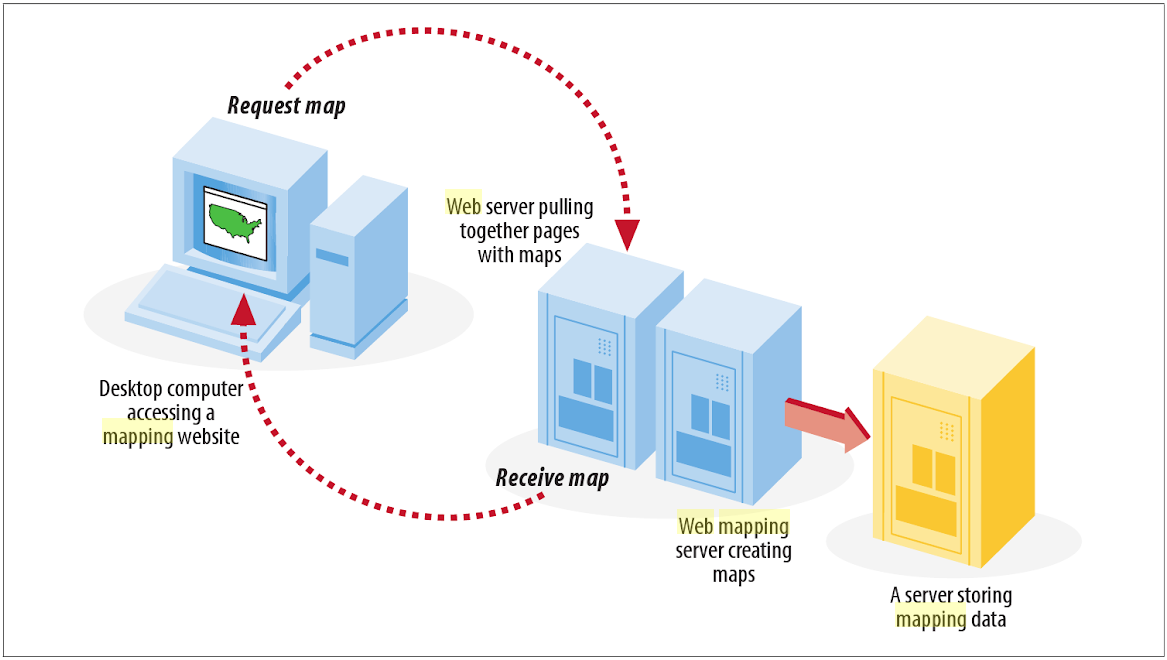
\includegraphics[width=1\textwidth]{../img/map-web-diagram.png}
%% ML: serverové části webové aplikace?
%% DT: vetu jsem preformuloval
	\caption{Diagram znázorňující základní části interaktivních mapových platforem a jejich interakci s uživatelem: \cite{web_mapping}}
	\label{fig:WPS_class_diagram}
\end{figure}

Na Obrázku 1 je znázorněn jednoduchý diagram, který popisuje fungování
interaktivní webové aplikace a jejích základních komponentů. Jedná především o tyto části:

\textit{Koncové zařízení} označované také jako webový klient,
využívající počítač, tablet, nebo mobilní telefon. Výsledná rychlost webové aplikace a její přinášený požitek dnes již není limitován tolik výpočetní
rychlostí klienta, ale především rychlostí internetového
%% ML: Vetsinu nutne komunikace
%% DT: Opraveno
připojení. Většinu nutné komunikace přitom zastává webový prohlížeč,
který pomocí \textit{request URL} získává informace z hostujícího
serveru, na kterém je webová aplikace reálně uložena.

\textit{Webový server -} přijímá požadavky od klienta a zastává nutnou
komunikaci mezi mapovým serverem a uložištěm dat. Na webovém serveru
je uložena aplikace a na vyžádání poskytuje obsah webové aplikace
%% ML: text nech nekym jeste precist, mas tam hrubky(!), silna kava, viz nize
klientovi.

\textit{Webový mapový server -} jedná se o program, který na základně
%% ML ta veta zni divne, zkus preformulovat
%% DT: změněno 
požadavků poslaných od webového klienta vytváří mapové kompozice. Data použitá mapovým serverem jsou v uložišti, do kterého má server přístup. Vytvořený mapový obraz je posléze odeslán zpět webovému klientovi. Mapových serverů existuje
%% ML: pridej odkazy na kapitoly
%% DT: doplněno
více. Těm nejvíce používaným se bude věnováno v kapitole \ref{ssec:mapove-platformy}.

\textit{Uložiště dat -} zde jsou fyzicky uložena všechna data potřebná k
vytvoření mapové kompozice, nebo její části. Jedná se o rastrová či vektorová
%% ML: mapova -> geograficka ?
%% DT: geografická
geografická data ve vhodném formátu, která dokáže webový mapový server
zpracovat. Dále jsou zde uložena metadata, která jsou nutnou součástí
%% ML: ta posledni data moc nedava smysl
%% DT: napsel jsem ji jinak
prostorových dat. Metadata popisují geografická data v předem dané struktuře \cite{web_mapping}.

Důležitou součástí každé webové mapové aplikace je samotná komunikace
mezi jednotlivými jejími komponenty. V následujících podkapitolách
bude brán zřetel převážně na komunikaci mezi webovým klientem a
webovým mapovým serverem. Konkrétně na metody, které jsou používané
%% ML: dalsi hrubka ...
%% ML: zkus posledni vetu preformulovat, v prvni vete mluvis o
%% protokolech, v druhe pise ``Tyto standardy''
%% DT: preformulovano a doplneno
pro získání mapového obrazu. Nejvíce používanou metodou, převážně v aplikacích s otevřeným kódem (viz. kapitoly \ref{sssec:mapserver}, \ref{sssec:geoserver}, \ref{sssec:qgis-server}), je použití protokolů poskytovaných mezinárodní standardizační organizací \textit{Open Geospatial Consortium (OGC)}.

\subsection{Open Geospatial Consortium}
\label{sssec:ogc}

Open Geospatial Consortium (OGC) je mezinárodní nezisková organizace
zahrnující komerční, vědecké, vládní a nevýdělečné organizace, které
se zabývají vytvářením kvalitních specifikací pro prostorová
data. Tyto specifikace jsou volně dostupné pro kohokoli za účelem
zlepšení sdílení prostorových dat po celém světě \cite{oqc_web}.

OGC specifikace jsou technické dokumenty detailně popisující rozhraní,
nebo kódování. Tyto dokumenty jsou dále použity na straně vývojářů k
%%% ML: vyvojari vetsinou nevlastni produkty :-)
%% DT: slovo "jejich" odstraněno
tvorbě produktů. Hlavním přínosem je skutečnost, že dva nezávisle
%% ML: standart -> standard (opakuje se v textu pravidelne)
%% DT: opaveno
vyvíjené programy používající OGC standardy by měly být vzájemně
kompatibilní \cite{oqc_web}. Celkem se jedná o více než 50
specifikací. Vzhledem k zaměření implementačního rámce této práce (viz. kapitoly \ref{sssec:initialization}, \ref{sssec:time-filtration}), budou konkrétněji popsány pouze následující:

\newpage
\begin{itemize}
\item\textit{Web Map Services (WMS)} - WMS nabízí jednoduché HTTP
  rozhraní pro posílání žádostí o georeferencovaný mapový obraz. Na
  základě WMS dotazu server odpoví odesláním rastrové mapy, která
  obsahuje požadované mapové prvky v daném výřezu (dlaždice).
	 
\item\textit{Web Map Tile Services (WTMS)} - princip fungování WMTS
  komunikace klient-server je obdobný jako u WMS. Rozdíl je však v
  tom, že v případě WMTS jsou požadované dlaždice již předem vytvořeny a uloženy
  v interní paměti serveru. Server je tedy nemusí při každém dotazu
  znovu vytvářet, což při velkém množství dotazů celý proces
  výrazně zrychlí.
\end{itemize}

\subsection{Web Map Services (WMS)}

%% ML: ten preklad mas odkud, zni priserne, vubec bych ho radeji
%% neuvadel, kdyz uz tak webova mapova sluzba
%% DT: preklad odstranen
WMS je mapová služba, která na základě poskytnutých
%% ML: s tim terminem ``mapa'' opatrne, kartografove by Ti to omlatili
%% o hlavu, tak alespon mapova kompozice.
%% ML: georeferencovana neni uplne korektni, georeference je soucasti
%% dotazu (bbox), vysledny obrazek uz referencovany neni, klient ho
%% ale umi korektne umistit, zna bbox
%% ML: standarta vetsinou visi nad hradem, knebo trenky ;-)
%% DT: georeferencovana mapa nahrazena mapovou kompozici
parametrů vytváří požadovanou mapovou kompozici. Mezinárodní standard dále
definuje \uv{mapový obraz} jako digitální vyobrazení geografických informací,
%% ML: preformulovat, produkt -> kompozici?
které je vhodné pro počítačové obrazovky a displeje. V případě mapové kompozice
%% ML: s terminem ``mapa'' bych setril, tak snad mapova kompozice?
%% ML: mapa obsahuje kartografickou omacku, tohle je pouze obrazova
%% kompozice geografickych dat, nic vic
%% DT: mapa opravena na mapovou kompozici
jako takové se tedy nejedná o data, ale o jejich produkt. Mapové kompozice 
%% ML: jsou poskytovány mapovych serverem v beznych obrazovych formatech...
%% DT: opraveno
jsou poskytovány mapovým serverem v běžných obrazových formátech, jako
např. PNG, GIF, nebo JPEG. Méně často se také jedná o vektorovou
grafiku ve formátech SVG, nebo WebCGM \cite{oqc_wms}.

Popisovaný standard definuje několik operací, každou s odlišným
%% ML: vraci vs. davaji
%% DT: opraveno
výstupem. Tyto operace vrací uživateli informace o
%% ML: myslis automobilovy servis? ;-) sluzbe!
samotné službě, nebo poskytují mapu či informace o zobrazovaných
mapových prvcích.

\begin{itemize}

%% ML: obecne poskytuje metadata
\item\textit{GetCapabilities} - operace vrací dokument obsahující popis 
  dat ve formátu XML.
  %% ML: souradnice -> rozsah v podporovanych souradnicovych systemech?
  %% DT: ok
  Pomocí GetCapabilities lze zjistit počet vrstev, jejich
  rozsah v podporovaných souřadnicových systémech atd.
	
\item\textit{GetMap} - jedná se o nejdůležitější operaci, protože
  %% ML: lepsi nez mapa
  jejím výsledkem je samotný mapový obraz. K jeho
  získání je potřeba poskytnout sadu parametrů, na základě kterých je
  %% ML: v?
  %% DT: mapovým
  mapovým serverem vytvořen. Těmto parametrům bude věnována následující
  %% ML: jaka
  %% DT: doplnena reference
  kapitola \ref{sssec:wms-param}.
	
\item\textit{GetFeatureInfo} - operace vrací informace o prvcích
  zobrazených na mapě.
	
\item\textit{GetLegendGraphic} - dle poskytnutých parametrů vytvoří
  tato operace legendu, kterou server vrátí jako obraz ve zvoleném
  formátu.
\end{itemize}

\subsection{Parametry WMS}
\label{sssec:wms-param}

Parametry obecně slouží ke specifikaci úkonu, který od mapového
serveru požadujeme. Jedná se tedy o vstupní informace na základě
kterých nám server odpoví. Parametrů je velké množství, některé jsou
používány vždy, některé jen velice ojediněle. Možnosti použití
%% ML: v textu pouzivas operace, presnejsi by byla asi ``dotaz''
parametrů se liší dle operace (requestu), kterou provádíme.

%% ML: mel bys uvest proc tak detailne rozepisujes parametry pro
%% GetMap
Níže uvedené parametry se vztahují pouze k operaci
\textbf{\textit{GetMap}}. Jsou zde uvedeny pouze nejdůležitější parametry a dále ty parametry, které se týkají implementační části práce (viz. kapitola \ref{sssec:time-filtration}). U operací jako \textit{GetCapabilities},
nebo \textit{GetFeatureInfo} může být popsaný význam parametrů odlišný.
V některých případech není možné parametr použít vůbec.

\begin{itemize}
\item\textit{VERSION} - specifikace verze WMS.
	
\item\textit{REQUEST} - výběr provedené operace (v případě požadavku o
 %% ML: mapu...
 %% DT: kompozice
  mapovou kompozici se jako \textit{REQUEST} parametr použije "GetMap").

%% ML: list -> seznam 
%% DT: seznam
\item\textit{LAYERS} - seznam oddělený čárkami obsahující názvy vrstev,
  které budou použity pro tvorbu mapy
	
\item\textit{SRS} - zkratka SRS v překladu znamená "geodetický
  referenční systém". Tímto parametrem je tedy určeno v jakém
  geodetickém referenčním systému jsou poskytnuté parametry
  např. BBOX.

%% ML: veta neda moc smysl, jinak Ti v textu casto chybi interpunkce
%% DT: preformulovano, nechám si to nekým opravit at s tim neni problem
\item\textit{BBOX} - jedná se o souřadnice výřezu, pro který je mapový obraz generován. Pro definování výřezu je třeba zadat
  %% ML: Pole -> Seznam
  %% DT: seznam
  souřadnice levého spodního a pravého horního rohu. Seznam souřadnic
  tedy parametr vypadá následovně "minX, minY, maxX, maxY".
	
\item\textit{FORMAT} - nastavení formátu výstupního souboru (mapového
  obrazu).
	
\item\textit{WIDTH} - celočíselná hodnota udávající šířku výsledné
  %% ML: mapa
  %% DT: mapová kompozice
  mapové kompozice v pixelech. Jinak řečeno se jedná o vzdálenost v pixelech 
  %% osa X
  osy X danou body \textit{BBOX} tj. vzdálenost minX a maxX. Osa Y odpovídá parametru \textit{HEIGHT}

\end{itemize}

Mezi další méně používané parametry patří např. \textit{EXCEPTIONS}, \textit{STYLES}, \textit{FORMAT}, \textit{ELEVATION}, \textit{BGCOLOR}, \textit{TRANSPARENT}, \textit{TIME} (jeho použití se liší viz. kapitoly \ref{sssec:mapserver}, \ref{sssec:geoserver}) \cite{oqc_wms}.

Výše uvedené parametry lze rozdělit na dvě části a to povinné a
nepovinné viz. tabulka:

\bigskip
\begin{table}[h!]
	\catcode`\-=12
	\centering
	\begin{tabular}{|c|c|}
		\hline
		parametr & povinný \\ \hline
		\hline
		VERSION & ano \\ \hline
		REQUEST & ano \\ \hline
		STYLES & ano \\ \hline
		SRS & ano \\ \hline
		BBOX & ano \\ \hline
		WIDTH & ano \\ \hline
		HEIGHT & ano \\ \hline
		TRANSPARENT & ne \\ \hline
		EXCEPTIONS & ne \\ \hline
		TIME & ne \\ \hline
		ELEVATION & ne \\ \hline
		BGCOLOR & ne \\ \hline
\end{tabular}
	\caption{Výpis parametrů a jejich povinnost použití: \cite{oqc_wms}}
	\label{tab:WPS_ExecuteRequest}
\end{table}

\subsection{Parametr TIME}
\label{sssec:time}

S ohledem na téma této práce a kapitoly \ref{sssec:mapserver}, \ref{sssec:geoserver} je vhodné přiblížit si parametr
\textit{TIME} podrobněji a popsat způsob jeho použití a možnosti,
které nabízí.

Dle OGC je formát parametru \textit{TIME} dán normou ISO 8601:1988(E),
která rozšiřuje normu ISO 8601. Oproti té jsou přidány další
specifikace\cite{oqc_wms}:
\begin{itemize}
\item Syntax pro datové kolekce. Jejich začátek, konec a periodické
  opakování.
\item Definice speciálních znaků pro vyjádření sedmi dní v týdnu.
\item Možnost zadání data před rokem 1 našeho letopočtu a to až do
  časově vzdálených geologických období (milióny a miliardy let v
  minulosti).
\end{itemize}

Základní časový formát ISO 8601:1988(E) rozšířené normy umožňuje
specifikovat časový formát až na úroveň tisícin sekund. Ne pro každou
hodnotu je však vyžadována takováto přesnost. Proto lze formát upravit
tak, že jsou odstraněny zpřesňující číslice.

\noindent
Základní formát vypadá následovně:

\begin{verbatim}
ccyy-MM-ddThh:mm:ss.SSSZ
\end{verbatim}

\noindent
A jeho zjednodušená forma pro vyjádření hodnoty s přesností na dny:

\begin{verbatim}
ccyy-MM-dd
\end{verbatim}

\newpage
\noindent
V ukázkách časových formátů jsou použita jednotlivá označení:

\begin{itemize}
	\item cc \textit{2 číslice století}
	\item yy \textit{2 číslice rok}
	\item MM \textit{2 číslice měsíc}
	\item dd \textit{2 číslice den}
	\item hh \textit{2 číslice hodina}
	\item mm \textit{2 číslice minuta}
	\item ss \textit{2 číslice sekunda}
	\item SSS \textit{3 číslice milisekunda}
\end{itemize}

\begin{itemize}
	\item T \textit{slouží k oddělení hodnot určující den a hodnot určující čas uvnitř dne}
	\item Z \textit{slouží k definici časového pásma vztaženému ke koordinovanému světovému času UTC}
\end{itemize}

Speciální znaky pro zadávání dnů v týdnu jsou: 'MON', 'TUE', 'WED',
'THU', 'FRI', 'SAT', 'SUN'. Pravěká období se definují např: M150
\textit{150 mil. let před Kristem (období Jura)}, K18 \textit{pozdní
  Doba ledová}

\newpage
\section{Webové mapové platformy}
\label{ssec:mapove-platformy}

Mapových publikačních platforem existuje v dnešní době velké
%% ML: jsou -> byly?
%% DT: byly
množství. Mohou být přizpůsobeny účelu za kterým byly vytvořeny, nebo
%% ML: Né zni divne, zkus tu vetu preformulovat.
%% DT: opraveno
konkrétním vstupním datům se kterými pracují. Podpora pro práci s časoprostorovými daty tedy není integrovaná ve všech. Tato
skutečnost je zároveň způsobena tím, že časoprostorová data nejsou
podporována všemi mapovými servery. Právě podpora na straně webového
mapového serveru je při tvorbě mapové publikační platformy
%% ML: neeee -> nikoliv
%% DT: nikoliv
klíčová, nikoliv však nutná.
 
%% ML: Veta ``jednotlive...'' je kostrbata, nedava moc smysl, preformulovat
%% DT: spojil jsem dve vety do jedne, protoze se duplikovaly
V této kapitole jsou představeny konkrétní webové mapové servery,
%% ML: posledni veta, tez preformulovat
%% DT: preformulovano
a dále je popsán jejich způsob podpory časoprostorových dat. Na závěr některých podkapitol je dále přidána ukázka webové mapové platformy využívající daný mapový server.

\subsection{MapServer}
\label{sssec:mapserver}

\begin{figure}[h!]
	\centering
	
\includegraphics[width=0.4\textwidth]{../img/mapserver-logo.png}
        %% popisek, zdroj
    \caption{Logo MapServer: \cite{mapserver_about}}
	\label{fig:mapserver-logo}
\end{figure}
\bigskip

MapServer je platforma s otevřeným kódem, která byla vytvořena pro
publikaci prostorových dat a interaktivních mapových aplikací. Byla
vytvořena v devadesátých letech na Minnesotské univerzitě. V té době se
%% ML: mas nekde OSGeo vysvetleno?, tak alespon poznamka pod carou zde
%% DT: doplneno
jednalo o jeden z prvních podporovaných projeků organizací OSGeo\footnote{\textit{OSGeo} je nevládní nezisková organizace s cílem  podporovat a prosazovat společný vývoj otevřených geoinformačních technologií a dat \cite{osgeo}}. Je
nutno podotknout, že MapServer není a ani nebyl navržen jako
%% ML: organizace? agenturou?
%% DT: agenturou
stoprocentní GIS systém. Důvod jeho vzniku je dán potřebou agentury
NASA, která hledala způsob jakým zprostředkovat satelitní snímky
%% ML: je napsan
%% DT: opraveno
veřejnosti. MapServer je napsán v jazyce C a podporuje všechny hlavní
operační systémy jakou jsou Windows, Linux a Mac OS X
\cite{mapserver_about}.

\bigskip
\noindent
\textbf{Podpora časových dat}

Od verze 4.4 je v MapServeru přidána podpora, která dokáže
%% odkaz na kapitolu o parametru time
%% DT: doplneno
interpretovat WMS parametr TIME (viz. kapitola \ref{sssec:time}) obsahující časovou hodnotu. MapServer
%% ML: dotazu
%% DT: opraveno
tuto hodnotu zpracuje a v dotazu vrátí odpovídající mapový obraz.

%% ML: urcite najdes lepsi slovo nez ``selektovat'' ;-)
%% DT: vybírat mapové prvky
K tomu, aby bylo možné vybírat mapové prvky jednotlivých vrstev pomocí atributu
TIME, musí každá vrstva obsahovat následující metadata
\cite{mapserver_about}:

\begin{itemize}
\item\textit{wms-timeextent} - povinná hodnota obsahující interval
  časových hodnot, které vrstva obsahuje. Tento interval lze zjistit
  pomocí operace \textit{GetCapabilities}.
\item\textit{wms-timeitem} - povinná hodnota obsahující název záznamu
  v databázi, ve kterém jsou časová data uložena.
\item\textit{wms-timedefault} - nepovinná hodnota určující implicitní
  hodnotu v případě, že časová hodnota pro daný záznam chybí.
\end{itemize}

\noindent
Záznam obsahující vrstvu s časoprostorovými daty vypadá následovně:

\begin{verbatim}
LAYER
	NAME "earthquakes"
	METADATA
	"wms_title"    "Earthquakes"
	"wms_timeextent" "2004-01-01/2004-02-01"
	"wms_timeitem" "TIME"
	"wms_timedefault" "2004-01-01 14:10:00"
	"wms_enable_request" "*"
	END
	TYPE POINT
	STATUS ON
	DATA "quakes"
	FILTER (`[TIME]`=`2004-01-01 14:10:00`)
	CLASS
	..
	END
END
\end{verbatim}

\bigskip
\noindent
\textbf{Formáty časových dat a syntaxe}

Výhodou použití MapServeru je jeho podpora dalších časových formátů,
které nejsou v normě ISO 8601:1988(E), používané pro operaci
\textit{WMS TIME}, definovány. Ke specifikování validních časových
formátů je možné pro každou vrstvu definovat \textit{wms-timeformat}

\begin{verbatim}
"wms_timeformat" "YYYY-MM-DDTHH
\end{verbatim}

%% ML: dotazu, ta veta mi nedava moc smysl, zkus preformulovat
%% DT: preformulovano
Dotaz s parametrem \textit{TIME} umožňuje přesně specifikovat
mapové prvky, které bude vytvořený mapový obraz obsahovat. Tímto způsobem je možné vybírat mapové prvky vrstvy pro specifické datum, nebo časový interval. MapServer
%% ML: s hodnoty?
%% DT: zmenena formulace vety
podporuje následující syntax (časové hodnoty jsou uvedeny ve formátu
'YYYY-MM-DD'):

\begin{itemize}
\item TIME=2004-10-12 \textit{pro jednu konkrétní hodnotu atributu.}
\item TIME=2004-10-12, 2004-10-13, 2004-10-14 \textit{pro více
    konkrétních hodnot.}
\item TIME=2004-10-12/2004-10-13 \textit{pro jeden konkrétní interval
    hodnot.}
\item TIME=2004-10-12/2004-10-13, 2004-10-15/2004-10-16 \textit{pro
    sjednocení více intervalů.}
\end{itemize}

\bigskip
\noindent
\textbf{Princip podpory časoprostorových dat}

%% ML: request -> dotaz
%% DT: opraveno
Princip fungování dotazu s parametrem \textit{TIME} je velice
snadný. Po té co MapServer přijme request, převede parametr
\textit{TIME} na parametr \textit{FILTER}. Tento parametr má na vstupu
název atributu obsahujícího časové hodnoty. Atribut je uložený v metadatech
časové vrstvy\cite{mapserver_about}. Další hodnotou je pouze převedená
hodnota časového parametru. V praxi vypadá filtr následovně:

\bigskip
\begin{itemize}
%% ML: selektovani -> vyber
%% DT: výber
	\item Pro výběr mapových prvků s konkrétní hodnotou
atributu, např. \textit{2004-10-12} hodnotu pro parametr 
\textit{FILTER} převede  na \textit{`[time-item]` eq `2004-10-12`}
	\item Pro selektování mapových prvků s konkrétním intervalem
hodnot, např. \textit{2004-10-12/2004-10-13}, interval pro parametr
\textit{FILTER} převede na \textit{(`[time-item]` ge `2004-10-12`) AND
(`[time-item]` le `2004-10-13`)}
\end{itemize}

%% ML: OGR neni format... (!), cela ta veta patri spise do poznamky
%% pod carou, kdyz uz
%% DT: poznamka odstranena, v kontextu prace neni dulezita

\bigskip
\noindent \textbf{Webové mapové platformy}

Webová mapová platforma zobrazující vývoj písčité pláže \textbf{Gay
Stand Sands} (\url{http://spatial.mtri.org/stampsands/}) využívá možnost
selekce časových dat. Její zvláštností však je, že k tomu není
použit parametr \textit{TIME}. Jelikož se jedná o malé množství
časových epoch, jsou tyto epochy rozděleny do jednotlivých vrstev s pojmenováním
podle časového filtru. Při requestu na konkrétní rok se tedy z
mapového serveru vrací konkrétní vrstva. Tento způsob je zvolen z
důvodu nekonzistence rastrových dat, která byla pořizována mezi lety
1938 až 2016.

\begin{figure}[h!]  \centering
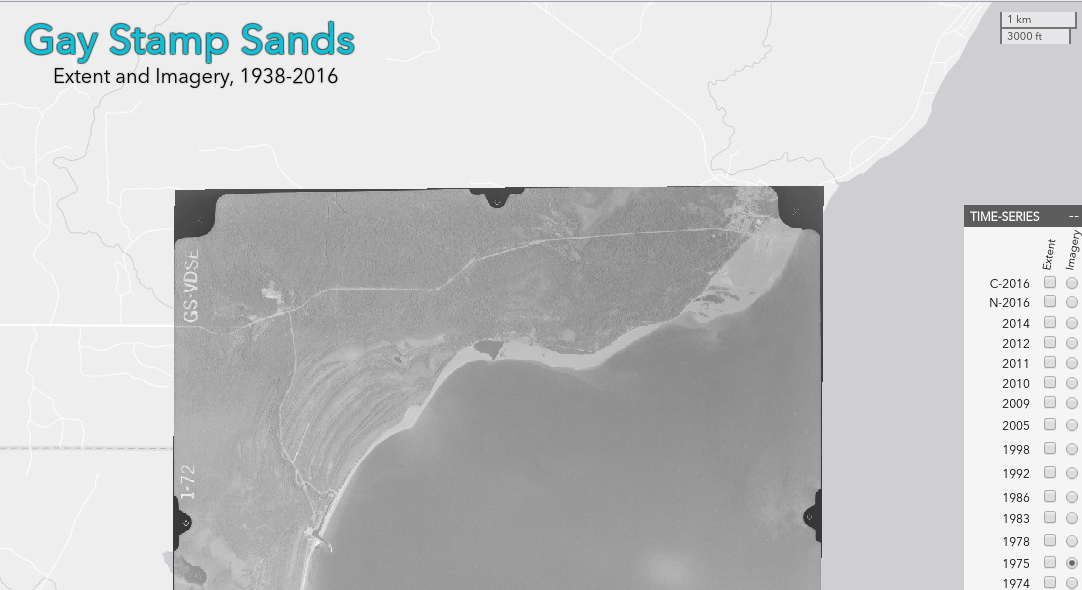
\includegraphics[width=1\textwidth]{../img/gay-sands.png}
        %% ML: screenshot nezni moc cesky, ukazka treba
        %% DT: ukazka
	\caption{Ukázka zobrazující webovou platformu Gay Stand
Sands a její uživatelské rozhraní}
	\label{fig:gay-sands}
\end{figure}

\newpage
\subsection{GeoServer}
\label{sssec:geoserver}

\begin{figure}[h!]  \centering

\includegraphics[width=0.4\textwidth]{../img/geoserver-logo.png}
	\caption{Logo GeoServer 
	\cite{geoserver-layer-edit}}
	\label{fig:geoserver-logo}
\end{figure} \bigskip

Stejně jako u MapServeru se jedná o serverový program s otevřeným
kódem. GeoServer je napsán v jazyce Java a umožňuje, na základě
otevřených standardů poskytovaných organizací OGC (viz. kapitola \ref{sssec:ogc}), sdílet a upravovat
%% ML: opravdu vsech?, co je hlavni?
%% DT: zaver vety odstranen
geografická data.

GeoServer vznikl v roce 2001 v neziskovém technologickém inkubátoru
\textit{The Open Planning Project} ve městě New York. V době vzniku bylo
hlavním cílem vytvoření sady nástrojů, které umožní větší vládní
průhlednost. Jako první nástroj vznikl právě GeoServer. Pomocí něj
mohla být veřejnost lépe zapojena do vládních záležitostí, především
územního plánování.

\begin{figure}[h!]  \centering
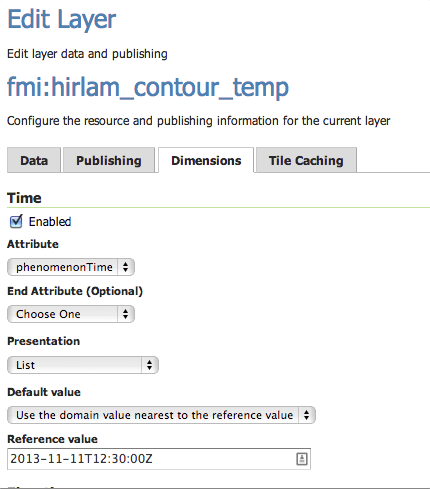
\includegraphics[width=0.6\textwidth]{../img/geoserver-layer-edit.png}
%% ML: popisky bezne zacinaji na velke pismeno\\
%% DT: vsude opraveno
	\caption{Záložka konfigurace časové vrstvy na GeoServeru
\cite{geoserver-layer-edit}}
	\label{fig:geoserver-layer-edit}
\end{figure}

\bigskip
\noindent

\textbf{Podpora časových dat}

Podpora časoprostorových dat na straně GeoServeru je velmi podobná té v
MapServeru. GeoServer podporuje v operaci \textit{GetMap} atribut
\textit{TIME}. Pro jeho použití je nutné mít správně nastavenou
vrstvu, která časová data obsahuje.

Nejjednodušším způsobem nastavení vrstvy je využití webového rozhraní
%% ML: nemel bys pouzivat cisla obrazku ``na pevno'', ale jako
%% dymamicky odkaz, navic bude potom v PDF i proklik, to se mozna tyka
%% i ostatnich obrazku (?)
%% DT: vsude dodelano
pro Geo\-Server viz. obrázek \ref{fig:geoserver-layer-edit}. V záložce \textit{Dimensions} je
nutné nastavení. V případě nastavení časové vrstvy je potřeba nejprve
zaškrtnout políčko \textit{Time Enabled}. Další nastavení je
následující \cite{geoserver-layer-edit}:

\begin{itemize}
	\item \textit{Attribute} - zde je nutné vybrat atribut, který
obsahuje časovou složku. Na základě něj jsou zjištěny časové
hodnoty. Volba atributu je možná pouze pro vektorové vrstvy.
	\item \textit{End Attribute} - jedná se o nepovinné
pole. Pomocí \textit{End Attribute} je nastavena horní hranice
intervalu hodnot, pro které je daný mapový prvek zobrazován.
	\item \textit{Presentation} - nastavení prezentace dat pro
\textit{GetCapabilities} operaci. Pokud jsou hodnoty diskrétní, tak je
možné nastavit možnost \textit{List}, \textit{interval and resolution}
pro hodnoty v intervalu s daným krokem, nebo \textit{continuous
interval} pro souvislý interval hodnot. Možnost \textit{List} je
vhodná například pro aplikace využívající animace, přičemž jeden časový
okamžik odpovídá jednomu snímku animace.
	\item \textit{Default value} - jedná se o hodnotu zastupující data, která pro zvolený atribut neobsahují žádnou časovou
hodnotu. Existuje několik možností jak \textit{Default value} zvolit:
	\begin{itemize}
		\item \textit{smallest domain value} - uloží nejnižší
hodnotu časového atributu
		\item \textit{biggest domain value} - uloží nejvyšší
hodnotu časového atributu
		\item \textit{nearest to the reference value} - uloží
hodnotu časového atributu, která je nejblíže dané referenční hodnotě
(\textit{Reference value})
%% ML: interpunkce
%% DT: opraveno
		\item \textit{reference value} - uloží danou
referenční hodnotu tak, jak je. Není brán ohled na skutečnost, zda-li je její použití vhodné.
	\end{itemize}
	\item \textit{Reference value} - pole pro zvolení referenční
hodnoty sloužící při určení \textit{Default value}.
\end{itemize}

\bigskip
\noindent \textbf{Formáty časových dat a syntaxe}

%% ML: opet request...
%% DT: opraveno
\noindent Obecná syntaxe pro dotaz s konkrétní hodnotou parametru
\textit{TIME} vypadá následovně:

\begin{verbatim} TIME=<timestring>
\end{verbatim}

Parametr \textit{TIME} je při \textit{GetMap} requestu vždy aplikován
na všechny aktuálně aktivní vrstvy definované parametrem
\textit{LAYERS}. Vrstvy bez časové složky tedy nejsou parametrem
\textit{TIME} nijak ovlivněny.

Pro zobrazení jednotlivých časových hodnot, intervalu a více hodnot je
syntaxe následující \cite{geoserver-time}:

\begin{itemize}
	\item TIME=2004-10-12 \textit{pro jednu konkrétní hodnotu
atributu.}
	\item TIME=2004-10-12,2004-10-13,2004-10-14 \textit{pro více
daných hodnot.}
	\item TIME=2004-10-12/2004-10-13 \textit{pro jeden konkrétní
interval hodnot.}
	\item TIME=2004-10-12/2004-10-13,2004-10-15/2004-10-16
\textit{pro více intervalů.}
\end{itemize}

Na první pohled je vidět, že rozdíl v syntaxi je v porovnání s MapServerem 
minimální. Mapserver však nabízí navíc možnost specifikace relativních
časových intervalů. Namísto přesné specifikace začátku a konce
intervalu je možné specifikovat začátek, nebo konec intervalu a přidat
dobu jeho trvání. Začátek či konec intervalu je zadán stejným
formátem, který je zobrazen výše. Pro hodnotu aktuálního času je možné
časovou hodnotu nahradit slovem \textit{PRESENT}.

Syntaxe pro specifikaci relativních intervalů je
následující\cite{geoserver-time}:

\begin{itemize}
	\item TIME=2002-09-01T00:00:00.0Z/P1M \textit{pro interval
hodnot pokrývající celý měsíc září 2002. Pro celý den 1. září
2002 by bylo možné použít hodnotu} P1D.
	\item TIME=P1D/2010-12-25T00:00:00.0Z \textit{pro interval
hodnot pokrývající celý den 24. prosince 2010.}
	\item TIME=PT36H/PRESENT \textit{pro časový interval 36 hodin
v minulosti od aktuálního časového okamžiku.}
\end{itemize}

\bigskip
\noindent \textbf{Webové mapové platformy}

%% ML: URL bych mohli byt proklikavaci (\url{}), to se tyka i
%% ostatnich odkazu
%% DT: opraveno vsude 
%nejsem si jist jestli je na GeoServeru \textbf{MetEye}
%% ML: nezapomen vyresit
(\url{http://www.bom.gov.au/australia/meteye}) je webová mapová platforma
zobrazující meteorologické observace a předpovědi pro celý australský
kontinent. Jedná se o interaktivní mapovou platformu vytvořenou
Australským úřadem pro meteorologii (Australian Bureaou of Metorology).

Webové rozhraní obsahuje panel s tématickými mapovými kompozicemi, 
který slouží ke specifikaci konkrétních meteorologických jevů. 
Zde lze vybrat typ předpovědi 
například vodní srážky, teplotu, sílu a směr větru atd. Mapové okno
%% ML: hrubku urcite najdes ;-)
%% DT: opravil jsem ji podle pravidla trenek na hrade
mimo standardních mapových prvků jako jsou legenda a grafické měřítko,
nabízí rovněž možnost zobrazení předpovědi počasí pro daný časový
okamžik. Toho je docíleno pomocí velice pěkně zpracované časové osy v
horní části mapového okna. Zde lze rovněž data po časových
úsecích animovat.

Rastrové vrstvy jsou filtrovány na základě parametru
\textit{TIMESTAMP}, který je vždy shodný u všech dlaždic. Vzhledem k
tomu, že pro jednotlivé předpovědi se mění pouze rastrové vrstvy, je
%% ML: hezke ceske slovo, a kdyz uz tak cache...
%% DT: nahrazeno mezipameti 
možné je na webovém serveru ukládat do mezipaměti a distribuovat ve formě dlaždic.

\begin{figure}[h!]  \centering
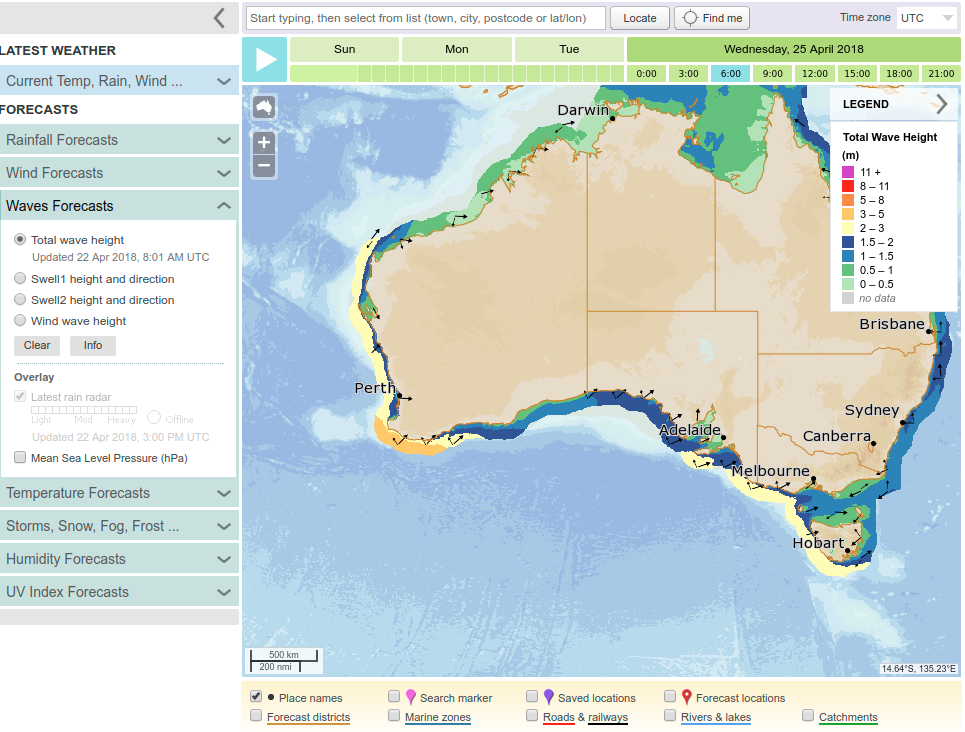
\includegraphics[width=0.67\textwidth]{../img/meteye.png}
%% ML: screenshot -> ukazka, zdroj
%% ML: doplneno
	\caption{Ukázka zobrazující webovou platformu MetEye}
	\cite{met-eye}
	\label{fig:met-eye}
\end{figure}

\textbf{Pennsylvania Cancer Atlas}
(\url{https://www.geovista.psu.edu/grants/CDC/}) je webová platforma
zobrazující výskyt rakoviny prostaty a tlustého střeva ve státě
Pensylvánie na severovýchodě USA. V tomto případě se jedná o webovou
mapovou aplikaci využívající software Adobe Flash Player, který se
spouští pomoci webového prohlížeče.

Uživatelské rozhraní nabízí tématickou mapu celého státu, která je
rozdělena na regiony. Ty jsou barevně zvýrazněny dle zastoupení
rakoviny v populaci. Pro každé období jsou dále vyhotoveny celostátní
statistiky, které jsou zobrazeny v grafech a v tabulce. Data jsou
zobrazována pro období jednoho až dvou let a pomoci jednoduchého
%% ML: selektovat
roletového menu je možné jednotlivě je selektovat nebo spustit
animaci. Pomocí panelu animace lze spustit animaci, ve které se
jednotlivá období střídají s předem daným časovým krokem. Ten dále
nabízí přeskočení na následující období a ukončení animování.

\begin{figure}[h!]  \centering
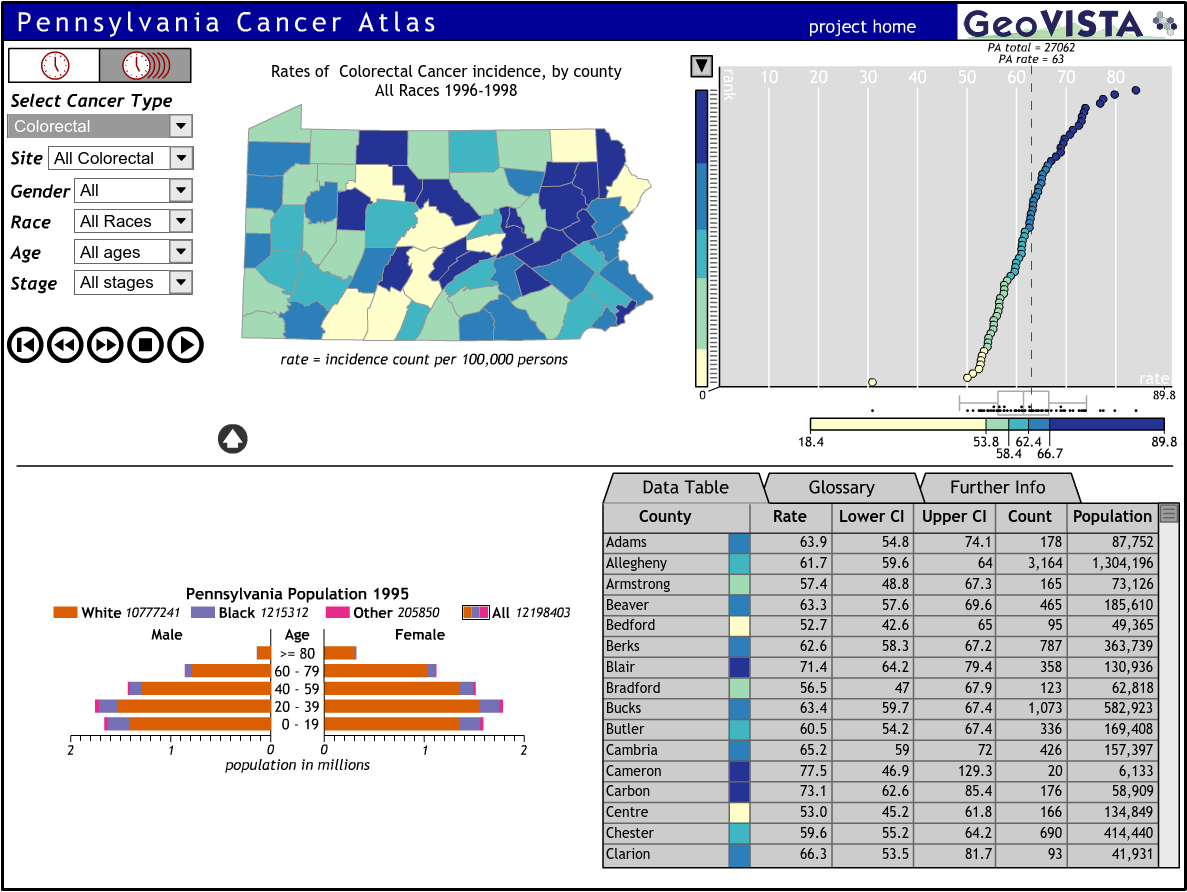
\includegraphics[width=0.8\textwidth]{../img/pennsylvania-cancer-atlas.png}
%% MK: ukazka, velke pismeno, vest zdroj
	\caption{Ukázka zobrazující webovou platformu Pennsylvania
Cancer Atlas a její uživatelské rozhraní s možností animace dle
časového období statistik}
	\cite{cancer-atlas}
	\label{fig:cancer-atlas}
\end{figure}
 
\newpage
\subsection{ArcGIS}

\begin{figure}[h!]  \centering

\includegraphics[width=0.4\textwidth]{../img/arcgis-logo.jpg}
	\caption{Logo ArcGIS}
	\cite{arcgis-logo}
	\label{fig:arcgis-logo}
\end{figure} \bigskip

ArcGIS je platforma obsahující řadu aplikací, které společně tvoří
geografický informační systém sloužící pro práci s prostorovými
daty. Nejedná se tedy o webový mapový server jako takový. ArcGIS je
%% ML: soukromy neni uplne vhodne slovo, treba proprietarni
%% DT: proprietarni
proprietární systém vytvořený firmou Esri (Environmental Systems Research
%% ML: mam pocit, ze ESRI vznikla podobne jako GRASS, nekdy na zacatku osmdesatych let
%% DT: cele jsem to preformuloval. Mam za to ye Esri vyikla takto brzy, ale ArcGIS jako takovy az pozdeji
Institute), která vznikla již v roce 1969. Nejznámějším produktem této společnosti je desktopová aplikace ArcGIS, která
se od doby svého vydání stala nejpoužívanějším komerčním softwarem na poli geografických informačních systémů \cite{arcgis-wiki}.

Pod ArcGIS patří mimo jiné aplikace pro webovou mapovou
publikaci. Jedná se o \textbf{ArcGIS Server}, \textbf{ArcGIS Online} a
\textbf{Portal for ArcGIS}.

\newpage
\subsection{ArcGIS Server}

Jedná o službu zahrnující mapování, geoprocessing, obrazové a síťové
analýzy, 3D data a možnost tvorby geografických prvků
\cite{arcgis-publishing-service}. Funkcionalita ArcGIS serveru se liší
dle balíčků, které na základě ceny omezují jeho možnosti.

\bigskip
\noindent \textbf{Podpora časových dat}
 
ArcGIS nabízí možnost práce s vrstvami obsahující časová data. K
tomu je nutné jednotlivé vrstvy ještě před jejich publikací
nastavit. V desktopové aplikaci k tomu slouží dialogové okno, které je
možné nalézt v nastavení vrstev.

\begin{figure}[h!]  \centering
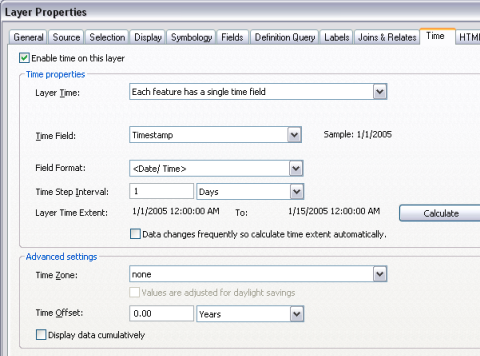
\includegraphics[width=0.8\textwidth]{../img/arcgis-layer-edit.png}
	\caption{Dialogové okno nastavení časové vrstvy v desktopové
aplikaci ArcGIS}
	\label{fig:arcgis-time-settings}
\end{figure}

K možnosti publikace je nejprve nutné zaškrtnout možnost \textit{Enable time
on this layer}. Tím bude vrstva jasně identifikována jako časová. Dále
je nutné specifikovat, jakým způsobem jsou časové hodnoty v datech
uloženy. Uloženy mohou být jako atributové pole pro vektorová data, nebo
jako rastrový katalog pro rastrová data. Nutné je rovněž nastavit
krok, jehož velikost by měla co nejlépe korespondovat s velikostí kroku, 
v jakém jsou jednotlivá data pořízena. Následující pole slouží k nastavení:

\begin{itemize}
	\item \textit{Time Properties} - v roletovém menu
\textit{Layer Time} je možnost zvolit, zda jsou data pouze v jednom
atributovém poli, nebo ve dvou. V případě dvou atributových polí 
obsahuje jedeno začátek a druhé konec časového intervalu. 
Konkrétní názvy atributů je dále nutné
zvolit z nabídky atributů pro příslušnou vrstvu. 
Poté je možné pomocí tlačítka \textit{Calculate}
vypočítat časový rozsah. Tato hodnota je posléze použita k
inicializaci časového posuvníku a rovněž k validaci časových dat. Po
výpočtu je vypsána doporučená velikost kroku časového posuvníku. Velikost
kroku lze případně změnit.
	
	\item \textit{Time Properties} - část s rozšířeným nastavením
není povinné nijak modifikovat. Obsahuje možnost specifikace časové
zóny pro použitá časová data. Takové nastavení je vhodné především pro
publikací více časových vrstev obsahující data z jiných časových
pásem. Pokud jsou jejich pásma specifikována, lze tato data snadno
kombinovat dohromady. Stejného výsledku lze také dosáhnout pomoci
nastavení časového posunu níže. V případě, že jsou některá časová data
pořízena v zemích používající změnu času na čas letní \textit{daylight
saving time}, nabízí ArcGIS tuto skutečnost u dat
specifikovat. Poslední možnost, kterou tato sekce nabízí je
\textit{Display data cumulatively} tedy kumulativní zobrazení dat. V
tom případě jsou zobrazena veškerá data mající počáteční časovou
hodnotu stejnou, nebo menší, než je hodnota aktuálně zvolená. Pokud taková data
mají nastavený konec časového intervalu je tato hodnota ignorována.
\end{itemize}

Takto nastavené vrstvy lze publikovat na ArcGIS server a pomocí
webových mapových servisů vytvářet požadované mapové obrazy. K jejich
finálnímu použití je však nutné mapový projekt publikovat na
server. Proces publikace již žádné dodatečné nastavení pro vrstvy
obsahující časová data neobsahuje, proto se mu tato kapitola věnovat
nebude.

\bigskip
\noindent \textbf{Formáty časových dat a syntaxe}

Jak již bylo upřesněno výše, časové hodnoty jsou podporovány ve třech datových
typech. Datový typ podporující datum, textový řetězec a číselná
hodnota. Pro nižší výpočetní náročnost je doporučeno maximálně využívat 
datové typy podporující datum. V případě textových řetězců je
podporováno 13 formátů a v případě číselných hodnot se jedná o 4
formáty \cite{arcgiq-data-types}.

\subsection{ArcGIS Online}

ArcGIS Online nabízí uživatelům publikování projektu přímo do cloudové
služby spravované společností ArcGIS. Nejedná se tedy o webový mapový server, ale o mapovou publikační platformu.
Způsob publikace je velice jednoduchý. V případě ArcGIS Online si není potřeba instalovat žádný software, nutné
je pouze vytvořit účet. Nabízené jsou dva hlavní typy
publikace. Jejich použití závisí na konkrétním použití aplikace. Pro
větší projekty je poté vhodná také jejich kombinace
\cite{arcgis-publishing-service}:
\begin{itemize}
	\item \textit{Feature services} - slouží především pro
publikaci atributů, mapových symbolů a dalších informací. Tyto mapové
objekty bývají často zobrazeny spolu s podkladovou mapou.
	\item \textit{Tiled map services} - jak již název napovídá,
jedná se o sadu předem generovaných mapových snímků, které jsou
serverem distribuovány ve formě mapových dlaždic. Ty mohou být pro
zvýšení výkonu aplikace drženy v mezipaměti serveru, odkud jsou přímo
dostupně přes jejich URL.
\end{itemize}

\bigskip
\noindent \textbf{Podpora časových dat} Stejně jako předchozí produkt
\textit{ArcGIS server}, tak \textit{ArcGIS online} nabízí taktéž
podporu pro práci s časoprostorovými daty. Nastavení se však liší a
vzhledem k již definovanému uživatelskému rozhraní jsou možnosti
použití rovněž omezeny na předem dané nástroje.

K tomu, aby mohla být daná vrstva označena jako časová, musí splňovat
dvě základní podmínky. Vrstva musí být typu \textit{feature layer},
\textit{map image layer}, \textit{imagery layer}, to jsou typy vrstev
podporující časové animace. Druhou podmínkou je označení konkrétní
vrstvy jako \textit{time enabled} tedy jako vrstvu podporující časová
data. Ověření podpory časových dat lze provést v \textit{map viewer} v
detailu vrstvy. Pro označení vrstvy jako časové je nutné provést kroky
popsané v podkapitole 2.4 (sekce Podpora časových dat). Pokud vrstva
splňuje obě podmínky a je označena jako viditelná zobrazí se ve spodní
části mapového prohlížeče nástroj pro správu časové vrstvy.

\begin{figure}[h!]  \centering

\includegraphics[width=0.8\textwidth]{../img/arcgis-online-time-slider.png}
	\caption{Nástroj pro správu časových vrstev}
	\label{fig:arcgis-time-slider}
\end{figure}

%vice detalneji? moznost obrazku a popisu detailniho nastaveni
casoveho nastroje Nástroj obsahuje časovou osu s posuvníky, tlačítka
pro vytvoření animace a tlačítko časového nastavení \textit{time
settings}. Po rozkliknutí tlačítka časového nastavení se zobrazí
dialogové okno, které umožňuje konfiguraci časové osy. Nastavení
dovoluje pro účely animace vrstvy změnit dobu trvání jednoho
snímku. Dále je možné omezit časovou osu jen na daný časový
interval. Implicitně je interval definován jako minimální a maximální
časová hodnota sjednocení intervalů časových hodnot pro všechny
vrstvy. V případě že není nastaveno kumulativní zobrazení dat, je
možné nastavit velikost intervalu pro který se v daný okamžik časová
data zobrazují.

Nastavení v detailu vrstvy rovněž umožňuje časový nástroj pro vrstvu
podporující časová data deaktivovat.

\newpage
\subsection{QGIS server}
\label{sssec:qgis-server}

Jedná se o mapový webový server s otevřenými daty implementující
pokročilé mapové prvky pro tvorbu tématických map. Zdrojový kód je
napsaný v programovacím jazyce C++, jsou v něm však podporované
zásuvné moduly psané jazykem Python, které umožňují rychlé a efektivní
vývoj nových komponent serveru a jeho rozšíření. V QGIS serveru jsou
implementovány standarty definované organizací OGC WMS 1.3, WFS 1.0.0
a WCS 1. Jeho vývoj byl podporován projekty Evropské unie Orchestra a
Sany a dále městem Uster ve Švýcarsku \cite{qgis-server}.

Výhoda použití QGIS serveru spočívá v použití stejné logiky jako u
desktopového QGIS. Pro vytváření map jsou použity stejné vizualizační
knihovny, které zároveň aplikují kartografická pravidla. To ve
výsledku znamená, že mapy publikované na webové publikační platformě s
použitím QGIS serveru budou vypadat stejně jako v desktopovém QGIS.

\bigskip
\noindent \textbf{Podpora časových dat}

QGIS server oproti ostatním zmíněným systémům nijak podporu pro data s
časovou složkou nepodporuje. Filtrace dat na základě parametru
\textit{TIME} tedy není možná.

Pro výše zmíněnou výhodu Qisquick platforma QGIS server používá. V
Druhé části práce bude popsáno jakým způsobem je možnost práce s
časoprostorovými daty s použitím QGIS serveru implementována.

\newpage
\subsection{Zhodnocení} V předešlých kapitolách byly popsány jednotlivé
principy a postupy práce s časoprostorovými daty pro rozdílné mapové
servery a mapové publikační platformy. Již na první pohled je zřejmé
že i přes dílčí rozdíly jsou ve všech aplikacích použity podobné
principy a pravidla.

Níže uvedená tabulka obsahuje porovnání publikačních platforem mezi 
sebou. Již na první pohled je zřejmé, že podpora časoprostorových dat ve 
volně dostupném software,
jako například MapSever a Geoserver se od sebe liší minimálně. Na 
druhou stranu licenční software v podobě ArcGIS Serveru a ArcGIS 
Online jsou od volně dostupných značně odlišné.
Vždy záleží na uživateli, zda-li preferuje otevřený zdrojový kód s širokou komunitou lidí v pozadí, nebo raději komerční software s obsáhlým uživatelským 
rozhraním. V Případě ArcGIS Online je 
použití pro mapovou publikaci nejjednodušší. Není zde nutná žádná 
instalace software, což z této platformy dělá ideální nástroj především 
pro méně zkušené uživatele.

\begin{table}[h]
	\centering
	\begin{tabular}{ | l| *6c | }
		
		  \multicolumn{1}{c}{vlastnost} & 
		  \mcrot{1}{l}{60}{MapServer} &
		  \mcrot{1}{l}{60}{GeoServer}& 
		  \mcrot{1}{l}{60}{ArcGIS Server} &   
		  \mcrot{1}{l}{60}{ArcGIS Online}  \\
		  
		  \midrule 
		  \midrule

		  možnost selekce na základě konkrétních hodnot i intervalů 
		  &  x & x & x &  \multicolumn{2}{c}{x} & \\
		  široká podpora časových formátů 
		  &  x & x & x &  \multicolumn{2}{c}{x} & \\
		  možnost nastavení časových vrstev v uživatelském
		  rozhraní 
		  &  - & x & x &  \multicolumn{2}{c}{x} & \\
		  časová hodnota mapového prvku může být interval 
		  &  - & x & x &  \multicolumn{2}{c}{x} & \\
		  nabídka časové hodnoty v případě, neexistujícího záznamu
		  &  - & x & x &  \multicolumn{2}{c}{x} & \\
		  užívající OGC standarty 
		  &  x & x & - &  \multicolumn{2}{c}{-} & \\
		  software s otevřeným kódem 
		  &  x & x & - &  \multicolumn{2}{c}{-} & \\
		  software s otevřeným zdrojovým kódem 
		  &  x & x & - &  \multicolumn{2}{c}{-} & \\
		  podpora časových pásem 
		  &  - & - & x &  \multicolumn{2}{c}{x} & \\
		  široká podpora datových typů 
		  &  - & - & x &  \multicolumn{2}{c}{x} & \\
		  bez nutnosti instalace softwaru
		  &  - & - & - &  \multicolumn{2}{c}{x} & \\
		  přímá integrace nástrojů pro práci s časoprostorovými
		  daty
		  &  - & - & - &  \multicolumn{2}{c}{x} & \\
		  
		\bottomrule
	\end{tabular}
	\caption{Výpis parametrů a jejich povinnost použití: \cite{oqc_wms}}
	\label{tab:WPS_ExecuteRequest}
\end{table}


 

\newpage
\part{Platforma Gisquick}
\newpage

\section{Úvod do Gisquick}

Gisquick je webová mapová publikační platforma s otevřenými daty. Jejím
účelem je snadné a rychlé publikování projektů vytvořených v programu
QGIS, které je možné posléze prohlížet na webovém rozhraní platformy
Quisqick.
Celá platforma se skládá z několika komponentů (jejich obecné fungování
je popsáno v kapitole \ref{sssec:fungovani-platforem} ). Komponenty jsou
následující.

\subsection{Komponenty}
\label{sssec:gisquick-komponenty}


\begin{itemize}
\item\textit{Gisquick plugin} - jedná se o zásuvný modul pro
program QGIS, pomocí kterého je možné existující projekt
publikovat. Publikace je nutná pro pozdější použití projektu
na platformě Gisquick. Během samotné publikace si může každý
uživatel projekt nastavit tak, aby zobrazovaný předmět zájmu
přesně odpovídal jeho požadavkům (možnost selekce jednotlivých
vrstev, nastavení maximálního a minimálního měřítka,
atd.). Gisquick plugin pracuje zcela odděleně od ostatních
komponentů a jeho výstupem je složka obsahující všechny použité
vrstvy, uložený projekt ve formátu .qgs a metadatový soubor. Ten
obsahuje nastavení provedené během procesu publikace a dále popis
projektu. Metadatový soubor je použit pro potřeby webového klienta.
\item\textit{webový server} - webový server zpracovává
dotazy z webového klienta ve formě OGC standardů (viz. kapitola
\ref{sssec:ogc}). Následně odpovídá například ve formě mapových
obrazů. Na straně webového serveru je použit aplikační rámec Django,
který je stejně jako Gisquick plugin psaný v jazyce Python.
\item\textit{QGIS server} - jedná se o webový mapový server
na základě kterého jsou vytvářeny mapové obrazy. Použití
QGIS serveru je dáno skutečností, že veškeré mapové prvky
zde vytvořené korespondují svým vzhledem s prvky vytvořenými
v QGIS desktopové aplikaci. Díky tomu si může být uživatel
jistý tím, že publikovaný projekt bude věrně odpovídat jeho
původnímu projektu.
\item\textit{webový a mobilní klient} - klient uživateli nabízí
uživatelské rozhraní celé aplikace, ve kterém se může
orientovat a pomocí kterého interaguje s webovým serverem a tak
mění zobrazovaný obsah. Právě této části spolu s Gisquick
pluginem byla je v této práci věnována největší pozornost.
\end{itemize}

\subsection{Uživatelské rozhraní}

\begin{figure}[h!]
\centering
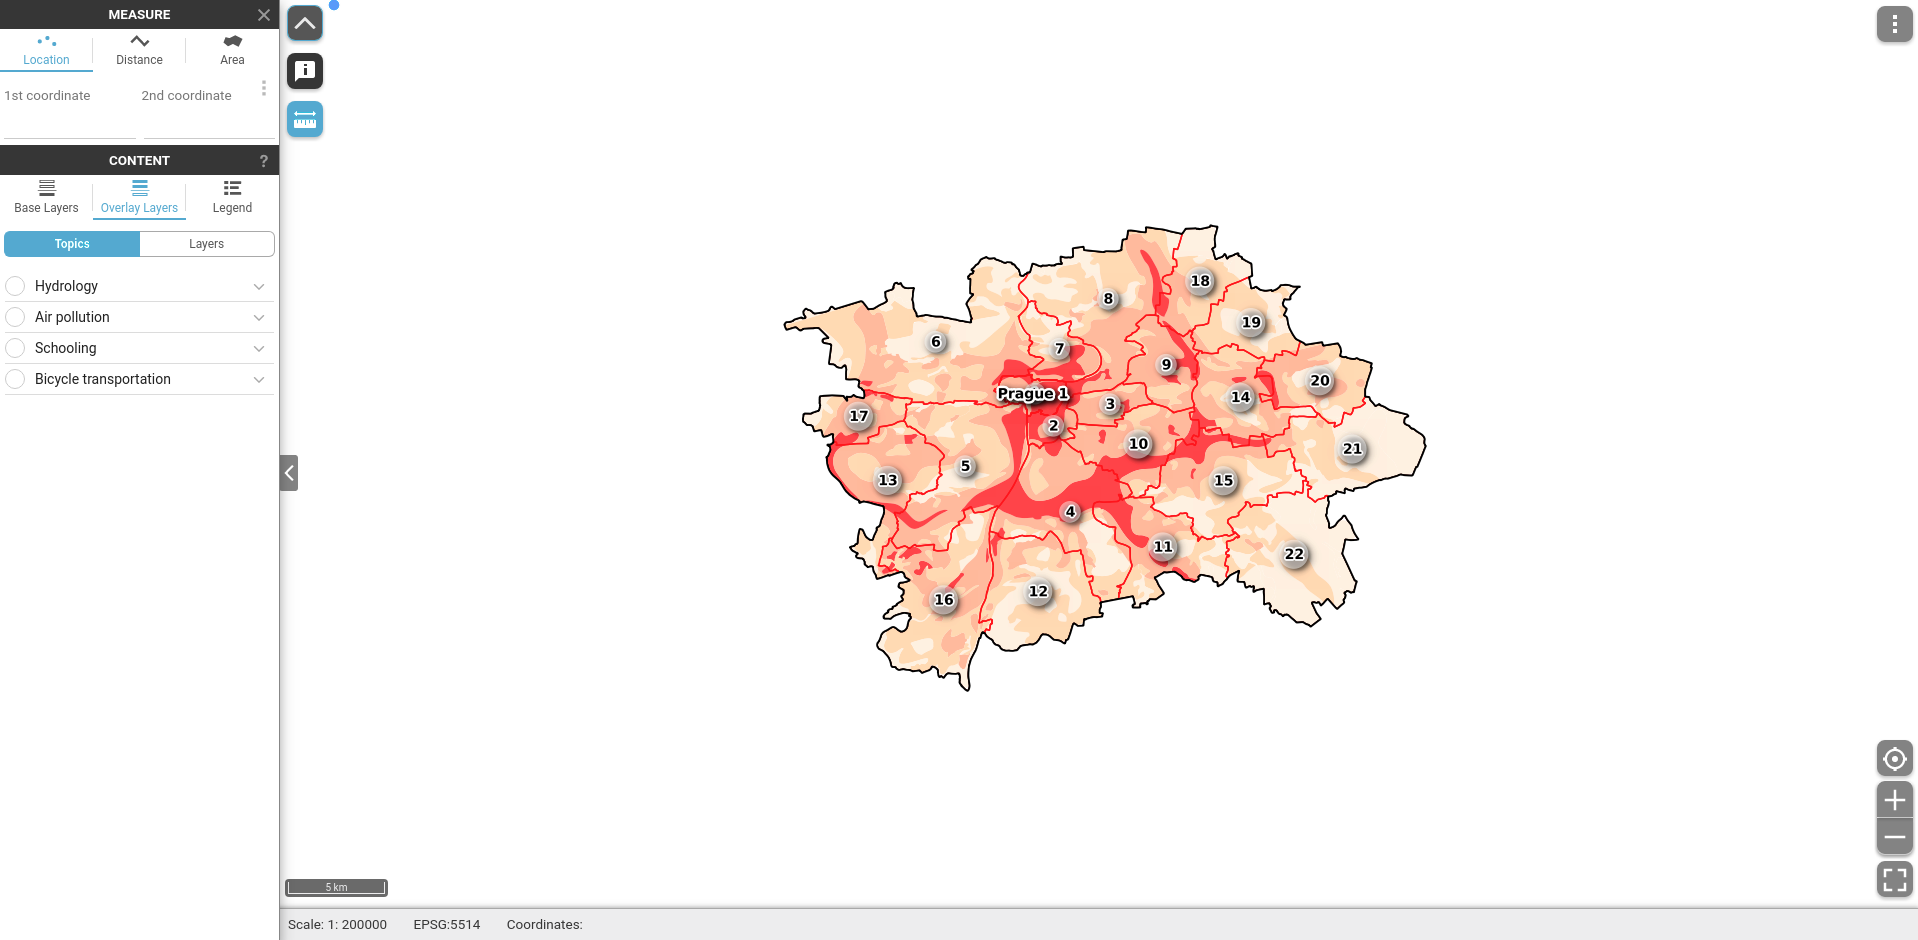
\includegraphics[width=0.9\textwidth]{../img/gisquick_ui.png}
\caption{Ukázka uživatelského rozhraní platformy
Gisquick\cite{gisquick-prague}}
\label{fig:gisquick-prague}
\end{figure}

Obrázek výše zachycuje webové uživatelské rozhraní platformy
Gisquick. Jedná se o sadu velice jednoduchých a intuitivních nástrojů
sloužících pro snadnou orientaci v publikovaném projektu, filtraci
jednotlivých částí a provádění jednoduchých operací. Například
měření vzdáleností na mapě.

Uživatel má být schopný rychlé a intuitivní orientace jak v projektu,
tak v samotné webové aplikaci. K tomu slouží postranní menu se správou
vrstev spolu s menu nástrojů, které je v obrázku \ref{fig:gisquick-prague}
rozbaleno. V horní postranního menu části je právě aktivovaný
nástroj sloužící k zjišťování souřadnic, měření vzdáleností
a ploch. Hlavní část je věnována interaktivní mapové kompozici. Ta
poskytuje možnost změny velikosti a polohy výřezu zobrazovaného území.

\begin{figure}[h!]
\centering
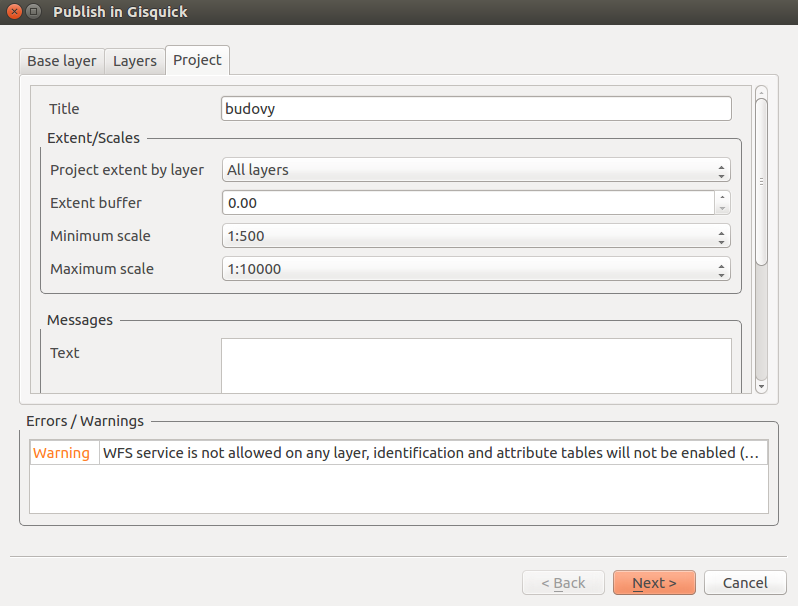
\includegraphics[width=0.7\textwidth]{../img/gisquick_plugin.png}
\caption{Ukázka uživatelského rozhraní Gisquick pluginu pro QGIS}
\label{fig:gisquick-plugin}
\end{figure}

\newpage
Gisquick plugin pro QGIS rovněž disponuje uživatelským rozhraním, kde
pomocí jednoduchého dialogového okna jsou nabízeny možnosti nastavení
pro export vrstev. Jeho první část je rozdělena na tři záložky a
stavovou řádku, ve které se jsou vypisována chybová hlášení. V
první záložce \textit{Base layer} je možno nastavit podkladové vrstvy
jako například Open Street Map, nebo Binq mapy. V další záložce
\textit{Layers} je možno nastavit které vrstvy budou publikované. Při
implementaci podpory pro časoprostorová data bylo nastavení v této
záložce rozšířeny o další možnosti. Tomuto rozšíření se bude
práce věnovat detailněji v dalších částech. V poslední záložce je
obecné nastavení projektu. Další okno slouží k nastavení \textit{topics}
nebo-li tématicky orientovaných vrstev \cite{gisquick-manual}. Předposlední
stránka obsahuje pouze souhrn publikovaného projektu. Poslední zobrazuje
výpis souborů, které se po zmáčknutí tlačítka \textit{Publish}
vytvoří. Ty je posléze nutné nahrát na Gisquick publikační server.

\newpage
\subsection{Použité technologie}

\begin{figure}[h!]
\centering

\includegraphics[width=0.8\textwidth]{../img/technologies.png}
\caption{Loga níže popsaných softwarů}
\label{fig:technoogies}
\end{figure}

\noindent
\textbf{Vue.js} - jedná se o moderní aplikační rámec s otevřeným kódem
napsaný v programovacím jazyce JavaScript, jehož první verze byla vydaná
začátkem roku 2014 Evanem You \cite{vue-history}. Jeho hlavní použití je
vývoj uživatelského rozhraní aplikací, tedy na straně webového klienta
(viz. kapitola \ref{sssec:fungovani-platforem}). Uživatelské rozhraní
je za pomoci Vue.js rozděleno na několik  komponent, kdy každá obsahuje
vlastní JavaScript, HTML a CSS skripty. Jednotlivé komponenty dělají kód
přehlednější a aplikace výkonově méně náročnější. Protože vždy
jsou použity jenom ty komponenty, které koncový uživatel v danou chvíli
potřebuje. Mezi další výhody Vue.js patří mimo práce s komponenty
jeho reaktivita, a úpravu objektového modulu dokumentu (DOM).

Původní verze webového klienta Gisquicku jsou psány za použití
aplikačního rámce AngularJS. V současné chvíli je však celý klient
vytvářen znovu za pomoci Vue.js. Z toho důvodu bylo rozšíření platformy
o podporu časoprostorových dat na straně klienta psáno právě ve Vue.js.

\newpage
\bigskip
\noindent
\textbf{PyQt} - PyQt je vazba pro programovací jazyk Python, která umožňuje
využití aplikačního rámce pro Qt aplikace. Vazby jsou vytvořeny ve formě
Python modulů a obsahují okolo jednoho tisíce tříd. Jedná se o kombinaci
výhod nabízející jednoduchost Pythonu a obrovské schopnosti Qt v jednom
celku. Díky tomu je možné jednoduše vytvářet grafické uživatelské
rozhraní přímo za pomocí Pythonu. PyQt je software s otevřeným kódem,
který byl vytvořen britskou firmou Riverbank Computing a je nabízen pod
dvojí licencí GNU GPL v3 a komerční licencí společnosti Riverbank
\cite{pyqt}.

\bigskip
\noindent
\textbf{Docker} - Docker je počítačový program s otevřeným
kódem umožňující zapouzdření (izolaci) jednotlivých aplikací do
kontejnerů. Vytvořený kontejner se nazývá \textit{Docker image}. Obecné
pravidlo je použití pouze jedné aplikace pro jeden Docker kontejner. Docker
image mohou být posléze spuštěny na jakémkoli hardwaru s operačním
systémem Linux, nebo Windows, na který je Docker program nainstalovaný. Tato
skutečnost má obrovskou výhodu pro nasazení aplikací do produkčních
serverů, jejich sdílení s dalšími uživateli, nebo vytváření
clusterů složených z dílčích aplikací. Po spuštění aplikace v
Docker kontejneru není vytvořen nový virtuální stroj, ale aplikace
v kontejnerech využívají hostující operační systém. Výhod tohoto
řešení spočívá v minimalizaci velikosti kontejneru.

Gisquick pro své komponenty (mimo Gisquick pluginu) v produkční
verzi využívá právě použití Docker kontejnerů. Tímto způsobem
je možné celou Gisquick platformu jednoduše spustit na lokálních
zařízeních. Vývoj je tak jednodušší, protože odpadá jakékoli
nastavování vývojového prostředí.

\bigskip
\noindent
\textbf{OpenLayers} - jedná se o knihovnu napsanou v programovacím
jazyce JavaScript, která umožňuje správu a vizualizaci map ve webových
prohlížečích. Jedná se o software s otevřeným kódem nabízející
široké rozhraní pro tvorbu geografických aplikací. OpenLayers byly
vytvořeny soukromou společností MetaCarta v roce 2005. Od roku 2007
spadají OpenLayers pod organizaci OSGeo.

\newpage
\section{Implementace nástroje pro Gisquick plugin}

V kapitole \ref{sssec:gisquick-komponenty} jsou zmíněny výstupy z Gisquick
pluginu. Jedná se o složku obsahující projekt ve formátu .qgs, data
použita v projektu a metadatový textový soubor. Hlavním cílem úprav
Gisquick pluginu bylo vytvoření jednoduchého uživatelského rozhraní,
které umožňuje definovat všechny potřebné parametry sloužící ve
webovém klientu k inicializaci nástroje pro práci s časovými daty. Tyto
parametry jsou během publikace pro jednotlivé vrstvy nastavené a dále
vepsané do metadatového souboru.

\subsection{Uživatelské rozhraní}
\label{sssec:plugin-ui}

\begin{figure}[h!]
\centering
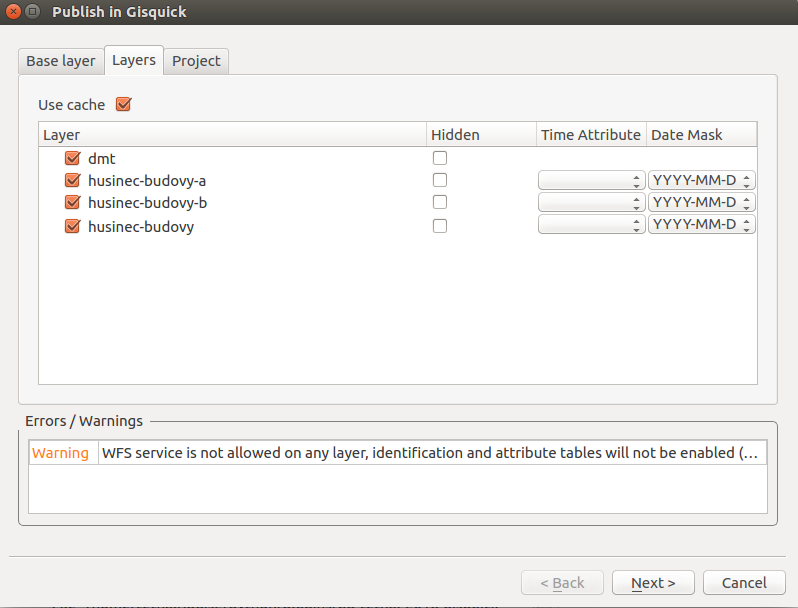
\includegraphics[width=0.9\textwidth]{../img/gisquick-plugin.png}
\caption{Nastavení vrstev v Gisquick pluginu}
\label{fig:gisquick-plugin-layers}
\end{figure}

Obrázek \ref{fig:gisquick-plugin-layers} zobrazuje dialogové okno publikace
projektu pomocí Gisquick pluginu. V prvním kroku publikace, v záložce
vrstvy \textit{Layers} je pro vektorové vrstvy přidáno nové nastavení. V
Případě rastrových, jako je například v obrázku zvolená vrstva dmt,
možnost nastavení časových vrstev není možná.

Ve sloupci \textit{Time Attribute} jsou v roletovém menu vypsány
všechny atributy každé vrstvy. Implicitní hodnota je prázdný textový
řetězec. Zde je nutné pro každou časovou vrstvu vybrat atribut, který
obsahuje časové hodnoty (dále jen časový atribut).

Sloupec \textit{Date Mask} obsahuje roletové menu s časovými formáty,
které určují jakým způsobem budou časová data na webovém klientu
zobrazena. Díky tomuto nastavení je možné, nehledě na formát časového
atributu, nastavit kterýkoli nabízený časový formát. V tomto formátu
budou zobrazeny časové hodnoty na webovém klientovy. V případě volby
formátu je nutné znát původní data. Přejde se tím situacím kdy
uživatel zvolí formát zobrazující pouze roky, zatímco původní data
budou v rozpětí jednoho dne.

Jestli jsou časové vrstvy dobře nastaveny, a výpočet proběhl korektně,
se lze v předposledním kroku publikace přesvědčit v souhrnu publikovaného
projektu (obrázek \ref{fig:publishing-summary}).

\begin{figure}[h!]
\centering
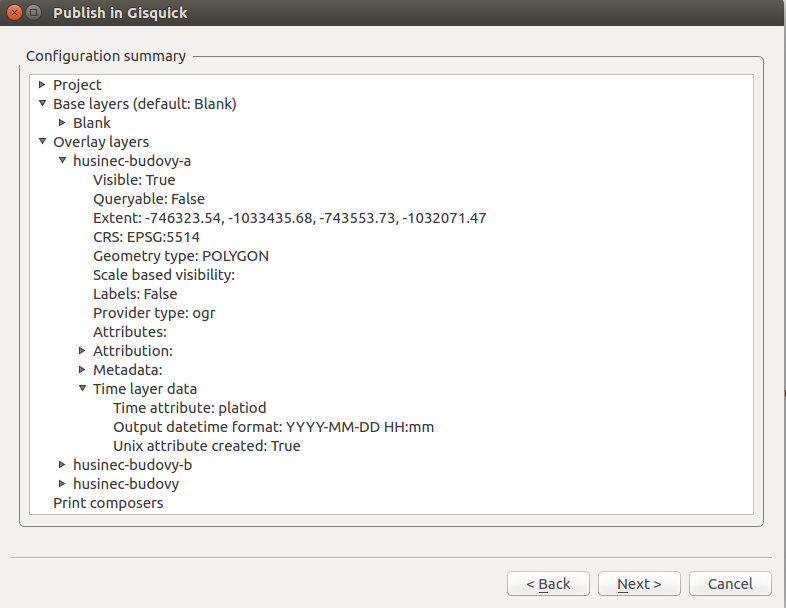
\includegraphics[width=0.9\textwidth]{../img/project-publishing-time-summary.png}
\caption{Souhrnu publikovaného projektu v Gisquick pluginu}
\label{fig:publishing-summary}
\end{figure}

\subsection{Funkcionalita}
\label{sssec:plugin-functionality}

Poté co uživatel v záložce \textit{Layers} nastaví všechny požadované
parametry může svou volbu potvrdit tlačítkem \textit{Next}, které
spustí výpočet a zobrazí další krok publikace.

Do výpočetního procesu se dostanou pouze ty vrstvy, které splňují dvě
podmínky. Jejich časový atribut musí existovat a nesmí být prázdným
textovým řetězcem. Tyto podmínky eliminují výpočet nad rastrovými
vrstvy. Dále zajistí to, že do výpočtu se dostanou pouze ty vrstvy,
které mají nastavený časový atribut. Tyto vrstvy jsou dále v textu
označovány jako časové.

Výpočet probíhá pro jednotlivé vrstvy splňující vstupní podmínky
totožně. Pro každou časovou vrstvu je volána metoda \verb|get_time_info|.

V prvním kroku metody \verb|get_time_info| je metodou
\verb|validate_time_attribute| vytvořena validační maska. Jedná se o pole,
které svou velikostí odpovídá počtu mapových prvků \textit{Features}
časové vrstvy. Každý prvek validační masky může nabývat různých
hodnot. Prvek může obsahovat časový formát textového řetězce, ve
kterém je časová hodnota uložena. Pokud však hodnota není v textovém
řetězci, nebo její časový formát textového řetězce neodpovídá
podporovaným formátům, je do daného prvku validační masky uložena
hodnota \textit{-1}. Podporované formáty jsou explicitně vypsány ve
zdrojovém kódu Gisquick pluginu v proměnné \verb|datetime_mask_array|.

Například pro časovou vrstvu obsahující šest prvků, kdy pouze pět
z nich má validní datum, a to ještě v odlišných časových formátech
může validační maska vypadat následovně:

\begin{verbatim}
[
'%Y-%m-%d',
'%Y-%m-%d',
-1,
'%Y-%m-%dT%H:%M:%S',
'%Y-%m-%dT%H:%M:%S',
'%Y-%m-%dT%H:%M:%S'
]
\end{verbatim}

Během vytváření validační masky jsou rovnou data kontrolována metodou
\verb|validate|. Díky tomu je možné zjistit jaká data maska obsahuje,
aniž by bylo nutné její jednotlivé prvky procházet. Po její vytvoření
jsou možné pouze tři scénáře popsané níže a zobrazené v obrázku
\ref{fig:plugin-chart}.

%!!!!!!!!!!!!!!!!!!!
%specialni znak

\begin{itemize}
\item\textit{Data nejsou validní} - znamená, že ani jedna
hodnota v zadaném časovém atributu nemá validní časový
formát. Validační maska v tomto případě obsahuje pouze hodnoty
\textit{-1}. Výpočet je tedy ukončen.
\item\textit{Data jsou validní a obsahují pouze jeden časový
formát} - v tomto případě je zjištěno, zda-li časový formát
neobsahuje speciální znak, který by jeho použití pro následnou
filtraci mapových prvků v původní podobě znemožnil použít.
\begin{itemize}
\item\textit{Obsahuje speciální znak} - zde se pokračuje
způsobem stejným jako v případě \textit{Data jsou
	validní, ale obsahují více časových formátů} popsaném
níže. Například při použití data v textovém formátu
'YYYY-MM-DDTHH:mm:SS', kdy je použit znak 'T' oddělující
datum a čas, nelze textový řetězec v parametru
\textit{FILTER} (viz. kapitola \ref{sssec:time-filtration})
použít.
\item\textit{Neobsahuje speciální znak} - časové hodnoty
jsou metodou \\* \verb|get_min_max_mask| za pomocí formátu,
zjištěného časového z validační masky, převedeny do
časového formátu \textit{UNIX TIME}. Z těchto hodnot
jsou poté zjištěny jejich maximální a minimální
hodnoty. Ty jsou součástí návratové hodnoty metody
\verb|get_min_max_mask|.
Pro získání časového formátu z validační masky je
použita metoda \verb|most_common|, která vybere nejvíce
zastoupený prvek v poli. Pro získání požadované hodnoty
je tedy nutné nejprve metodou \verb|remove_values_from_list|
odstranit záznamy obsahující hodnoty \textit{-1}.
\end{itemize}
\item\textit{Data jsou validní, ale obsahují více časových
formátů} - jedná se tedy o validní nekonzistentní data. Pro tento
případ slouží metoda \\* \verb|create_unix_time_attribute|, která
má návratovou hodnotu stejnou jako metoda \verb|get_min_max_mask|. K
tomu, aby časové hodnoty byly konzistentní, je nutné metodou
\verb|create_new_attribute| vytvořit nový atribut obsahující
hodnoty v jednotném formátu. Toho je docíleno pomoci validační
masky, kdy se jsou procházeny její jednotlivé hodnoty. Pokud
pro záznam existuje formát časového textového řetězce,
je jeho hodnota převedena do formátu \textit{UNIX TIME}. Ten
je následně uložen v novém atributovém sloupci metodou \\*
\verb|changeAttributeValues|. V případě časové hodnoty, která
není validní je pole prázdné. Z nově vytvořeného atributu
jsou dále určeny minimální a maximální hodnoty časového
atributu. V případě, že nový atribut již jednou vytvořen byl,
jsou jeho hodnoty pouze přepsány.
\end{itemize}

\begin{figure}[h!]
\centering
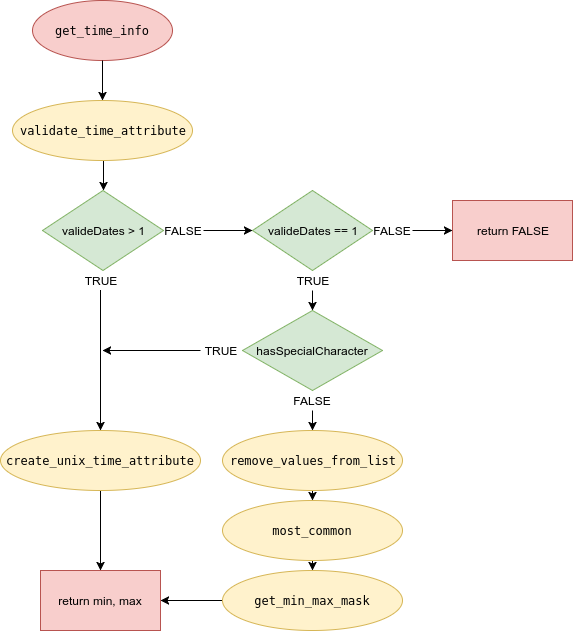
\includegraphics[width=0.8\textwidth]{../img/getTimeInfo.png}
\caption{Vývojový diagram publikace časové vrstvy}
\label{fig:plugin-chart}
\end{figure}

Posledním krokem je poté pouze export zjištěných hodnot do metadatového
souboru. Každé časové vrstvě je vypsán časový formát pro zobrazení
časových hodnot na webovém klientu. Dále název časového atributu,
minimální a maximální hodnota časového atributu ve formátu \textit{UNIX
TIME} a další parametry, které budou popsány a vysvětleny dále. V
případě, že data jsou validní a obsahují pouze jeden časový formát
je vypsán tento formát. Pokud tomu tak není a je použit pomocný atribut
s hodnoty ve formátu \textit{UNIX TIME}, je vypsán jeho název.

\subsection{Metadatový soubor}
\label{sssec:metadata}

Metadatový soubor (viz. kapitola \ref{sssec:gisquick-komponenty}, část
\textit{Gisquick plugin}) je textový soubor, který vniká publikací
projektu Gisquick pluginem. Obsahuje množství informací, které jsou
nutné pro správnou konfiguraci straně webového klienta.

Pokud jsou vrstvy při publikaci označeny jako časové a jejich data jdou
validní, jsou do nich vepsány následující hodnoty:

\begin{itemize}
\item\textit{unix} - parametr unix nabývá hodnoty \textit{TRUE}
v případě, že byl vytvořen pomocný atribut s časovými
hodnoty ve formátu \textit{UNIX TIME}. Slouží webovému
klientu k určení zda-li má k filtrování časové vrstvy
(viz. kapitola \ref{sssec:time-filtration}) použít daný formát
\textit{input\textunderscore datetime\textunderscore mask}, nebo
\textit{UNIX TIME}.
\item\textit{original\textunderscore time\textunderscore attribute}
- zde je uložen název časového atributu. Parametr slouží k
určení atributu při filtrování časové vrstvy (viz. kapitola
\ref{sssec:time-filtration}).
\item\textit{output\textunderscore datetime\textunderscore mask}
- obsahuje formát časového řetězce, který si uživatel
zvolil v roletovém menu \textit{Date Mask} (viz. kapitola
\ref{sssec:plugin-ui}). Tento parametr definuje formát, kterým
jsou zobrazeny časové hodnoty na straně webového klienta.
\item\textit{time\textunderscore values} - jedná se o pole
obsahující minimální a maximální hodnotu časového
atributu ve formátu \textit{UNIX TIME}. Na základě těchto
hodnot je na webovém klientu inicializovaný časový
posuvník (viz. kapitoly \ref{sssec:one-layer-filtration},
\ref{sssec:multiple-layers-filtration}).
\item\textit{input\textunderscore datetime\textunderscore mask} - tento
parametr je vytvořen pouze pokud není nutné vytvářet pomocný
atribut (viz. kapitola \ref{sssec:plugin-functionality}). Parametr
obsahuje formát časového řetězce zvoleného časového
atributu. Díky tomuto parametru může být pro potřeby filtrování
časové vrstvy převedena hodnota učená na časovému posuvníku
do stejného časového formátu v jakém je uložena (viz. kapitola
\ref{sssec:time-filtration}).
\item\textit{time\textunderscore attribute} - parametr
je vytvořen pouze pokud je nutné vytvářet pomocný
atribut obsahující hodnoty ve formátu \textit{UNIX TIME} a
obsahuje název tohoto atributu. Parametr slouží stejně jako
\textit{original\textunderscore time\textunderscore attribute}
k specifikaci atributu při filtrování časové vrstvy.
\end{itemize}

\newpage
\bigskip
\noindent

Níže je zobrazena ukázka části metadatového souboru. Ta obsahuje dvě
časové vrstvy, kdy každá z nich má odlišné parametry. Pro kompaktnost
ukázky zde parametry, které se netýkají implementovaného rozšíření,
zobrazeny nejsou:

\begin{verbatim}
{
"unix": false,
"time_values": [
1309471200.0,
1507672800.0
],
"input_datetime_mask": "YYYY-MM-DD",
"output_datetime_mask": "YYYY-MM-DD",
"original_time_attribute": "platiod",
},
{
"time_attribute": "UTconvert",
"unix": true,
"time_values": [
1309471200,
1507672800
],
"output_datetime_mask": "HH:mm",
"original_time_attribute": "platiod1",
}
\end{verbatim}

\newpage
\section{Implementace nástroje do webového klienta}
Webový klient obsahuje hlavní část implementace rozšíření pro podporu
časoprostorových dat. Jedná se o jednoduchý nástroj, který umožňuje
filtrovat mapové prvky jednotlivých časových vrstev na základě jejich
časového atributu. Časový interval je možné nastavit pomoci posuvníku,
nebo přímo pomocí kalendáře a hodinového ciferníku. Nástroj na
webovém klientu umožňuje dále vytvářet jednoduché animace. Uživatel
má možnost zmíněnou filtraci mapových prvků provádět pro jednotlivé
vrstvy, nebo pro více vrstev současně.

\subsection{Uživatelské rozhraní}
\label{sssec:gisquick-client-ui}

\begin{figure}[h!]
\centering
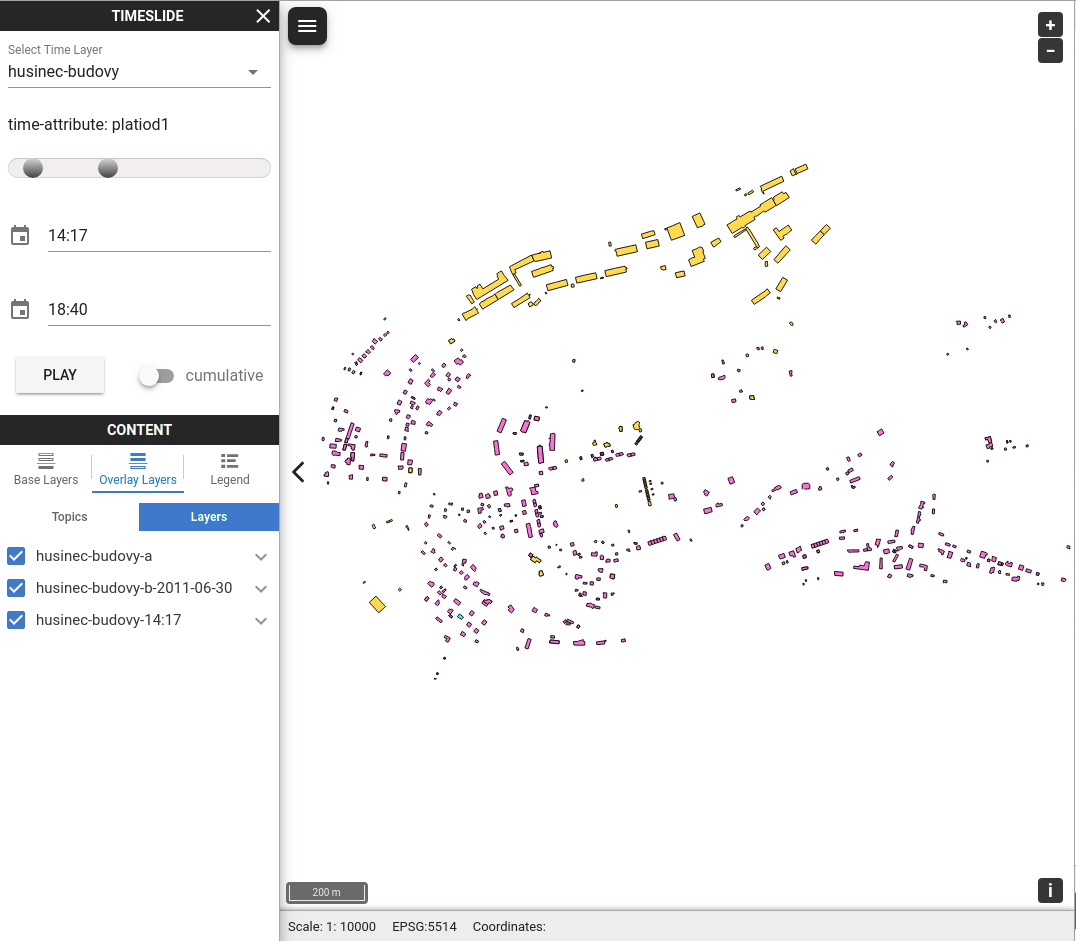
\includegraphics[width=1\textwidth]{../img/gisquick-time-tool.png}
\caption{Webové rozhraní Gisquick platformy s aktivovaným nástrojem
pro páci s časoprostorovými daty}
\label{fig:gisquick-client}
\end{figure}

Celý nástroj je ukrytý v postranním menu a obsahuje jen několik prvků,
které však uživateli poskytují velké množství operací. Všechny
jsou zobrazeny v obrázku \ref{fig:gisquick-client}. Od shora se jednotlivě
jedná o:

\begin{itemize}
\item\textit{roletové menu s výběrem časové vrstvy} - v
případě aktivace nástroje je toto pole jediný prvek, který
je uživateli zobrazen. Jako první krok je nejprve nutné vybrat
časovou vrstvu, která bude použita. Toho lze docílit pomocí
zmíněného roletového menu, které obsahuje všechny časové
vrstvy. Dále je zde možnost "All visible layers", která uživateli
umožňuje výběr všech viditelných časových vrstev.
\item\textit{jméno časového atributu} - tento prvek neumožňuje
uživateli jakoukoli interakci s nástrojem a má tedy čistě
informativní charakter. Je zde vypsán název časového atributu
vybrané vrstvy. Jeho existence je přínosná především v
případě, kdy projekt obsahuje více časových vrstev s odlišným
časovým parametrem. Při výběru možnosti "All visible layers" je
možné použít pouze vrstvy se stejným parametrem. Uživatel je tedy
tomto případě informován pro jaký parametr jsou vrstvy vybrány.
\item\textit{dvojitý časový posuvník} - jedná se posuvník
se dvěma
%%DT: nedokázal jsem přijít na lepší slovo, nez šoupátka
šoupátky. Díky němu je možné snadno a rychle mapové
prvky filtrovat. Uživatel tak ihned získá představu o jejich
rozmístění na časové ose. Minimum a maximum posuvníku odpovídá
minimu a maximu intervalu časových hodnot jednotlivé vrstvy. Pro
více vrstev se jedná o minimum a maximum sjednocení intervalů. Krok
je vždy určen jako jedna setina intervalu hodnot posuvníku.
\item\textit{časové štítky} - na dvou řádcích jsou dvě
textové pole s minimálním a maximálním datem filtrovaných
časových hodnot. Tato pole slouží k přesné definici
časového úseku. Každé z nich obsahuje integrovaný kalendář
s hodinovým ciferníkem pro určení hodnot. Časový formát
zobrazený v těchto polích je definován při publikaci projektu
(viz. kapitola \ref{sssec:plugin-ui}). Pokud formát neobsahuje
možnost zobrazení minut, nebo hodin, v tom případě se hodinový
ciferník nenabízí. Stejným způsobem není nabídnuta možnost
filtrování za pomoci kalendáře v případě, že časový formát
obsahuje jen hodiny, nebo minuty.
\item\textit{animační tlačítko} - tlačítkem \textit{PLAY}
je možné spustit animování aktivní časové vrstvy. Po jeho
aktivaci je vždy po jedné sekundě zvyšována hodnota horní hranice
intervalu časových hodnot a to o jeden krok posuvníku. Pokud je
animace aktivována změní se tlačítko na \textit{STOP}. Tím je
tak možné animování zastavit.
\end{itemize}

\subsection{Princip časové filtrace}
\label{sssec:time-filtration}

Jak bylo zmíněno v kapitole \ref{sssec:qgis-server}, QGIS server nepodporuje
v operaci \textit{GetMap} parametr \textit{TIME}. Z toho důvodu je nutné
použít obdobnou metodu, kterou používá MapServer, a to nahrazení
parametru \textit{TIME} parametrem \textit{FILTER}.

\noindent
Parametr \textit{FILTER} lze použít v operaci \textit{GetMap} následovně
\cite{qgis-service}:
\begin{verbatim}
http://myserver.com/?
REQUEST=GetMap
&LAYERS=mylayer1,mylayer2
&FILTER=mylayer1:"OBJECTID" = 3;mylayer2:'text' = 'something'&....
\end{verbatim}

Tato skutečnost dovoluje filtrovat časové vrstvy na základě jejich
časového atributu resp. jeho názvu a hodnoty. Lze tak filtrovat jednu
i více vrstev najednou. Za použití speciálních znaků jako jsou
\textit{‘AND’, ’OR’, ’IN’, ’=’, ’<’, ’>=’,  ‘>’,
’>=’, ’!=*,’(‘,’)’} lze rovněž filtrovat intervaly hodnot
a jejich sjednocení \cite{qgis-service}.

V implementovaném nástroji pro časovou filtraci je při filtrování použit
dvojitý časový posuvník. Proto je obsah parametru \textit{FILTER} vždy
tvořen jako textový řetězec, který v obecné formě vypadá následovně:

\begin{verbatim}
mylayer1:
"timeAttribute" >= 'lowerValue'
AND
"timeAttribute" <= 'upperValue'
\end{verbatim}

Parametr \textit{FILTER} podporuje hodnoty časového atributu v datovém
typu textového řetězce, nebo jako celé číslo. Pro zachování
konzistence výsledků filtrování je nutné, aby časový formát hodnoty
vstupující do parametru \textit{FILTER} korespondovaly s příslušným
formátem časového atributu. Z toho důvodu je při publikaci projektu
ve speciálních případech nutné vytvoření pomocného atributu
(\ref{sssec:plugin-functionality}). Ten obsahuje hodnoty časového atributu
převedeny do formátu \textit{UNIX TIME}. To dovoluje k časovým hodnotám
přistupovat jako k celým číslům. V případě časového filtrování
této vrstvy není tedy použit námi zvolený časový atribut, ale nově
vytvořený.

\subsection{Inicializace nástroje}

Pokud není volba \textit{Use cache} při publikování projektu vypnutá
(viz. obrázek \ref{fig:gisquick-plugin-layers}), používá Gisquick webový
klient pro zobrazování mapových vrstev předem vytvořených mapových
dlaždic uložených v mezipaměti serveru. Pro možnosti filtrace vrstev
na základě jejich časové hodnoty parametru však tento způsob nelze
aplikovat. Bylo by totiž nutné vytvořit mapové dlaždice pro všechny
možné časové intervaly a kombinace vrstev. Z toho důvodu je při aktivaci
nástroje pro práci s časoprostorovými daty použit \textit{Lifecycle Hook
Created}. Jedná se o funkci, která se spustí jakmile je Vue komponent
inicializován. V ní je původní instance třídy \textit{ImageLayer}
uložena do proměnné \textit{originalLayer} a skryta. Následně je
vytvořena instance nová, která obsahuje stejné mapové vrstvy jako
původní. Ta je poté nastavena jako aktivní. Pokud je nástroj vypnut
je použita původní instance a webový klient je tedy opět v původním
nastavení.

\subsection{Filtrace jedné časové vrstvy}
\label{sssec:one-layer-filtration}

První a také jediný krok, který lze po inicializaci časového nástroje
udělat je volba časové vrstvy. Zde je možno zvolit jednotlivé časové
vrstvy, nebo filtraci všech viditelných časových vrstev. Pokud je
vybrána možnost filtrace mapových prvků pouze jedné vrstvy, je tato
vrstva v případě jejího skrytí znovu zviditelněna. Následný postup
je popsán dále.

\bigskip
\noindent \textbf{Inicializace}

Nejprve nutná inicializace časového posuvníku. Na něm jsou závislé
další uživatelské prvky jako například \textit{časové štítky}
(viz. kapitola \ref{sssec:gisquick-client-ui}). Jeho minimální a maximální
hodnota je získána z metadatového parametru \textit{time\textunderscore
attribute} (viz. kapitola \ref{sssec:metadata}). Velikost kroku posuvníku
určena jako setina rozdílu jeho maximální a minimální hodnoty. Metoda
\verb|setSliderValue| inicializuje hodnoty šoupátek na jejich poslední
použité. V případě, že nebyla vrstva ještě filtrována, je hodnota
levého šoupátka rovna minimu časového posuvníku a hodnota pravého
šoupátka o krok časového posuvníku větší.

Stejně jako hodnoty parametru \textit{time\textunderscore attribute},
tak hodnoty šoupátek jsou v časovém formátu \textit{UNIX Time}, tedy
jako celočíselný datový typ. \textit{Vue.js} umožňuje nastavení
\textit{Watched Property}. Takto jsou nastavené proměnné hodnoty
šoupátek. Pokud se tedy jedna z hodnot změní je spuštěna metoda,
která provede převod původního celočíselného časového formátu
\textit{UNIX Time} do časového formátu \textit{output\textunderscore
datetime\textunderscore mask} zvoleného během publikace projektu
(viz. kapitola \ref{sssec:plugin-ui}, \ref{sssec:metadata}). Jakmile je tedy
časový posuvník inicializován, jsou ihned inicializovány i časové
štítky hodnotou v daném časovém formátu.

\bigskip
\noindent \textbf{Filtrace}
%\ref{appendix}
Způsob, jakým je aktualizována mapa na základě změny časových hodnot je
popsána v dokumentaci časového nástroje. Zde je popsán princip, kterým je
mapový obraz dle stávajícího nastavení časového nástroje aktualizován.

Při spuštění časové filtrace je v metodě \verb|updateSingleLayer|
provedeno několik po sobě jdoucích operací:
\begin{itemize}
\item\textit{detekce předem filtrovaných vrstev} - nejprve je
nutné zjistit, zda-li ostatní viditelné časové vrstvy již
filtrovány byly. V takovém případě je potřeba do parametru
\textit{FILTER} zahrnout nastavení předem filtrovaných
vrstev. Pokud by tak nebylo provedeno, z těchto časových
vrstev by byly zobrazeny všechny jejich mapové prvky. To
je provedeno metodou \verb|getFilterFromLayers|, která vrací
textový řetězec obsahující obsah parametru \textit{FILTER}
(viz. kapitola \ref{sssec:time-filtration}) časových vrstev,
které byly již předem filtrovány.
\item\textit{sestavení filtru pro danou vrstvu} - další krok
zahrnuje vytvoření obsahu parametru \textit{FILTER} pro právě
filtrovanou vrstvu. Tento krok se liší v závislosti na existenci
pomocného časového atributu s hodnoty ve formátu \textit{UNIX
TIME} (viz. kapitola \ref{sssec:plugin-functionality}). Parametr
\textit{unix} v metadatovém souboru (viz. kapitola
\ref{sssec:metadata}) obsahuje informaci o jeho vytvoření.
\begin{itemize}
\item\textit{unix = TRUE} - znamená to, že filtrace není
provedena nad hodnoty původního časového atributu, ale
pomocného atributu. Pro tuto kofiguraci je textový řetězec
sestaven pouze z parametrů poskytovaných metadatovým
souborem. Pro časovou hodnotu je přímo použita hodnota
posuvníku, která je v časovém formátu \textit{UNIX TIME}.
\item\textit{unix = FALSE} - v tomto případě je
nutné nejprve časové hodnoty převést z formátu
\textit{UNIX TIME} do textového řetězce, který
svým časovým formátem odpovídá formátu časového
atributu dané vrstvy. Formát pro záznamy časového
atributu je součástí metadatového souboru jako
\textit{input\textunderscore datetime\textunderscore mask}
(viz. kapitola \ref{sssec:metadata}). Sestavení textového
řetězce je poté obdobné jako v předchozím případě.
\end{itemize}
Na konci tohoto kroku jsou poté spojeny dohromady obsahy parametru
\textit{FILTER} z ostatních časových vrstev a nově vytvořený.
\item\textit{nastavení filtrované vrstvy} - tento krok je nezbytný
z několika důvodů. Je nutné uložit hodnoty časového posuvníku
v případě že vrstva bude v budoucnu filtrována znovu. Dále je
nutné uložit použitý obsah parametru \textit{FILTER}, který
je použit při filtrování ostatních časových vrstev. Jako
poslední věc je změněn název vrstvy tak, aby obsahoval její
jméno spolu s časovou hodnotou. Tímto způsobem uživatel ihned
ví, které vrstvy byly již filtrovány.
\item\textit{provedení operace GetMap} - v posledním kroku je
metodou \verb|updateParams| poslán požadavek na server obsahující
parametr \textit{FILTER} s obsahem složeným z filtru pro všechny
viditelné časové vrstvy. Server vrátí v odpovědi mapový obraz s
filtrovanými mapovými prvky, pomocí kterých je původní mapový
obraz nahrazen.
\end{itemize}

\begin{figure}[h!]
\centering
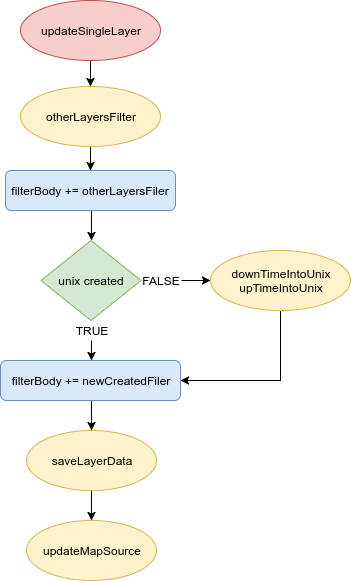
\includegraphics[width=0.5\textwidth]{../img/getSingleLayer.png}
\caption{Vývojový diagram filtrace více časových vrstev najednou}
\label{fig:single-chart}
\end{figure}

\subsection{Filtrace všech viditelných časových vrstev}
\label{sssec:multiple-layers-filtration}

Možnost selekce více vrstev je možné aktivovat v roletovém menu
obsahujícím jednotlivé časové vrstvy. Výběrem \textit{Select all
visible layers} je umožněno provádět filtraci mapových prvků pro
všechny viditelné časové vrstvy najednou.

\bigskip
\noindent \textbf{Inicializace}

Jednotlivé časové vrstvy mohou obsahovat navzájem odlišné
časové atributy, které v jistých případech nedovolují společnou
filtraci. Například pokud by projekt obsahoval dvě odlišné časové
vrstvy, kdy jedna by zachycovala časový průběh v intervalu jednoho dne
a druhá v intervalu jednoho roku. Výsledný krok časového posuvníku by
v takovém případě nebyl schopný postihnout nekonzistentní rozdělení
mapových prvků na časové ose. Z toho důvodu je při výběru možnosti
\textit{Select all visible layers} nejprve zjištěno, zda-li všechny
viditelné časové vrstvy mají zvoleny stejný, nebo odlišný časový
atribut. Tato zkutečnost je zjištěna metodou \verb|checkMultipleAttributes|,
která pro všechny viditelné časové vrstvy zjistí unikátní časové
atributy a uloží je do pole. Pokud takové pole obsahuje více, než jeden
prvek je zobrazeno další roletové menu ve kterém je nutné časový
atribut specifikovat.

Při inicializaci časového posuvníku je nutné brát v potaz
odlišné časové intervaly jednotlivých časových vrstev. Metoda
\verb|getSliderRange| postupně projde všechny viditelné
časové vrstvy mající zvolený časový atribut a z hodnot jejich
\textit{time\textunderscore values} (viz kapitola \ref{sssec:metadata}) určí
celkové maximální a minimální hodnoty. Tímto způsobem je zajištěno,
že všechny hodnoty časového atributu pro všechny časové vrstvy budou
náležet intervalu daného minimální a maximální hodnotou časového
posuvníku. Hodnoty šoupátek jsou nastaveny na minimální hodnoty
intervalu časového posuvníku, resp. na hodnotu, která je o časový
krok větší. Není přitom zohledňováno předchozí použití časových
vrstev při jejich filtraci tak, tako je tomu u fitrace jednotlivých vrstev.

Dále je nutné zajistit, aby časové hodnoty zobrazované na webovém
klientu, při filtraci více vrstev najednou, měly společný časový
formát. Časový formát je pro jednotlivé vrstvy definovaný v metadatovém
souboru (viz kapitola \ref{sssec:metadata}). Metoda \verb|setDateMask|
má za úkol mezi časovými formáty filtrovaných vrstev najít takový,
který poskytuje nejdetailnější zobrazení. Pokud tedy jedna z vrstev
má nastaveno zobrazování s podrobností minut, je její časový
formát upřednostněn. Metoda pro jednotlivé časové formáty nejprve
zjišťuje zda-li obsahují zároveň roky, hodiny a minuty. Pokud ano je
první nalezený formát použit. Pokud tomu tak není je hledán formát
obsahující alespoň roky. V případě, že ani takový není nalezen,
je použit časový formát první časové vrstvy.

Pro správné zobrazení kalendáře, hodinového ciferníků a
pro výběr hodnot časových štítků je nutné zjistit, jestli
nalezený časový formát obsahuje datum a čas. K tomu slouží metoda
\verb|maskIncludeDate|. Na základě jejího výsledku je skryta možnost
výběru časových hodnot pomocí kalendáře. Zobrazení hodinového
ciferníku je řešeno obdobně s tím rozdílem, že k detekci času v
časovém formátu je použito JavaScriptové metody \verb|includes|. Tato
metodika je provedena jak při výběru více časových vrstev, tak při
výběru jednotlivé vrstvy.

\bigskip
\noindent \textbf{Filtrace}

Princip a jednotlivé kroky samotné filtrace mapových prvků pro všechny
zobrazené časové vrstvy odpovídají popsanému principu pro filtraci
jednotlivých vrstev. Je zde však jedna podstatná změna při vytváření
obsahu parametru \textit{FILTER}. V metodě \verb|updateMultipleLayers| je
oproti metodě \verb|updateSingleLayer| přidán cyklus, který prochází
jednotlivě všechny viditelné časové vrstvy a zjišťuje jestli jejich
časový atribut je shodný s časovým atributem filtrovaných časových
vrstev. Dále je sestaven obsah parametru \textit{FILTER}. Pro každou vrstvu
mohou nastat dva případy:
\begin{itemize}
\item\textit{atribut není totožný} - pokud již byla
vrstva předem filtrována obsahuje použitý obsah parametru
\textit{FILTER}. Ten je v tomto případě zjištěn a
přidán do nově vytvářeného obsahu.
\item\textit{atribut je totožný} - časová vrstva je
filtrována a je tedy nutné sestavit obsah parametru
znovu. Tento princip je stejný jako v případě filtrace
jednotlivé vrstvy. Obsah parametru je rovněž přidán do
nově vytvářeného obsahu. Pro vrstvu jsou navíc uloženy
stejné hodnoty jako v případě filtrace jednotlivých
vrstev. Pokud by tedy vrstva byla znovu samostatně
filtrována, inicializuje se časový posuvník naposledy
uloženými hodnoty.
\end{itemize}
Pokud jsou všechny viditelné časové vrstvy zpracovány je nově vytvořený
obsah parametru \textit{FILTER} použit při operaci \textit{GetMap} stejným
způsoben jako u filtrace jednotlivé vrstvy.

\begin{figure}[h!]
\centering
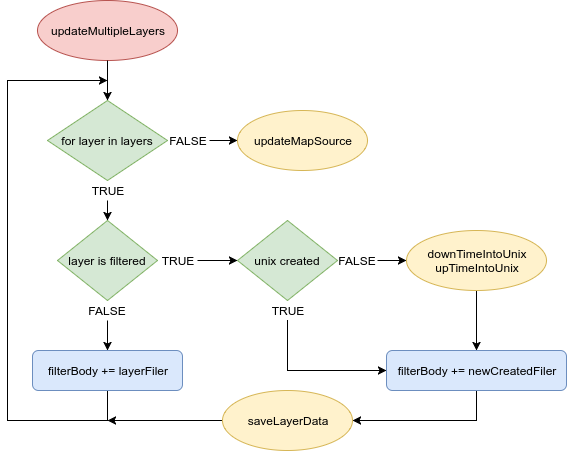
\includegraphics[width=0.9\textwidth]{../img/getMultipleLayers.png}
\caption{Vývojový diagram filtrace více časových vrstev najednou}
\label{fig:multiple-chart}
\end{figure}

\subsection{Animace filtrace}

Jak pro jednotlivé vrstvy, tak pro více vrstev najednou je možnost
provádět filtraci mapových prvků automatizovaně a vytvářet tak
jednoduché animace. K tomu slouží tlačítko \textit{PLAY} na spodní
straně nástroje viz. kapitola \ref{sssec:gisquick-client-ui}.

Jedná se o jednoduchou metodu \verb|animate|, která s prodlevou jedna
sekunda mění hodnotu časového posuvníku. Tato metoda pouze kontroluje
hodnotu proměnné \textit{animateStop}. Pokud je tato hodnota FALSE, je
volána metoda \verb|newFrame|. Metoda \verb|newFrame| při každém svém
zavolání zkontroluje hodnotu checkoboxu cumulative:
\begin{itemize}
\item\textit{cumulative = TRUE} - pokud je hodnota horního šoupátka
menší než maximální hodnota časového posuvníku, je zvýšena
o krok posuvníku. Pokud je vyšší, je zvýšena hodnota spodního
šoupátka.
\item\textit{cumulative = FALSE} - pokud je hodnota horního šoupátka
menší než maximální hodnota časového posuvníku, jsou zvýšeny
společně obě hodnoty šoupátek o krok časového posuvníku.
\end{itemize}
Po zvýšení hodnot je zavolána metoda \verb|getNewUrl| (viz. kapitola
\ref{sssec:one-layer-filtration}), která aktualizuje mapový obsah podle
nově nastavených filtrovaných hodnot. Nakonec v případě, že hodnota
\textit{animateStop = FALSE}, zavolá rekurzivně sama sebe s časovou
prodlevou jedna sekunda.

\begin{figure}[h!]
\centering
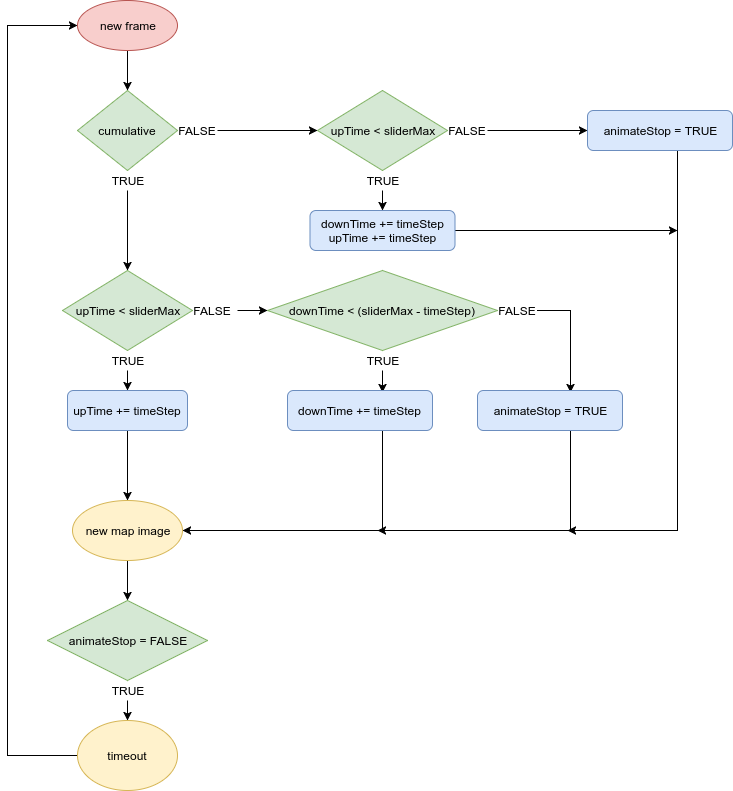
\includegraphics[width=0.9\textwidth]{../img/animate.png}
\caption{Vývojový diagram metody animate}
\label{fig:animate-chart}
\end{figure}

%
\newpage
\part{QGIS plugin pro Gisquick}
\newpage
\section{Principy publikace QGIS projektu}

\section{Implementace časových atributů}
\newpage
\necislovana{Závěr}
Hlavní cíle této práce byly dva. První spočíval v rešerši možných metod pro řešení podpory časoprostorových dat pro webové mapové publikační platformy obecně. Druhý cíl práce spočíval v implementování nástroje pro podporu zobrazování vektorových dat na publikační platformu Gisquick. Jednalo se o především o úpravy na straně Gisquick webového klientu a dále na straně zásuvného modulu pro QGIS.

Zásuvný modul byl doplněn o jednoduché uživatelské rozhraní umožňující snadné nastavení jednotlivých vrstev obsahujících časoprostorová data. Jedná se především o definování atributu obsahujícího časové hodnoty v nejrůznějších časových formátech. Na základě jeho definice jsou posléze dopočítány další parametry nutné na straně Gisquick webového klienta.

Nejvíce změn především z uživatelského hlediska bylo provedeno na již zmiňovaném webovém klientu. Zde byl přidán zcela nový nástroj, který na základě časové osy dává uživateli kontrolu nad výběrem zobrazovaných mapových prvků. Nástroj obsahuje různé způsoby určení časového intervalu pro selektování mapových prvků jedné, nebo více vrstev. Nástroj dále umožňuje vytvářet jednoduché animace. 

Způsob jakým byl jak samotný nástroj, tak změny zásuvného modulu implementovány úzce odráží poznatky získané během rešerše. Jedná se o funkční řešení převzaté z časové podpory pro MapServer a Geoserver. Stejnou mírou také o aplikované řešení z hlediska uživatelského rozhraní použité v produktech jako ArcGIS Server a ArcGIS Online.

I přes vytvoření plně funkčního nástroje, který nabízí příjemné uživatelské rozhraní a širokou škálu možností selekce, nabízí nástroj možnosti budoucího vývoje. Nejdůležitější pro časový nástroje především z hlediska jeho komplexnosti by byla implementace pro zobrazování časoprostorových rastrových vrstev. Dále na straně zásuvného modulu pro QGIS se jedná o zjednodušení validace dat a následného výpočtu, které by bylo přínosné především pro projekty s větším objemem dat. V této práci byla validace dosti benevolentní. Ta na úkor časově náročnějšího výpočtu dovoluje uživatelům použití dat s nekonzistentním časovým formátem. Na straně webového klienta jde především o grafickou stránku nástroje, která vzhledem k jeho možným budoucím změnám nebyla brána jako důležitá.


\newpage
\necislovana{Seznam zkratek}

\begin{tabular}{ll}
\textbf{GIS}& Geographic information system\\
\textbf{QGIS}& Quantum GIS\\
\textbf{WMS}& Web Map Service\\
\textbf{URL}& Uniform Resource Locator\\
\textbf{OGC}& Open Geospatial Consortium\\
\textbf{WMTS}& Web Map Tile Service\\
\textbf{PNG}& Portable Network Graphics\\
\textbf{GIF}& Graphics Interchange Format\\
\textbf{JPEG}& Joint Photographic Experts Group\\
\textbf{SVG}& Scalable Vector Graphics\\
\textbf{WebCGM}& Web Computer Graphics Metafile\\
\textbf{XML}& Extensible Markup Language\\
\textbf{SRS}& Spatial Reference System\\
\textbf{BBOX}& Bounding Box \\
\textbf{ISO}& International Organization for Standardization \\
\textbf{WCS}& Web Coverage Service\\
\textbf{CSS}& Cascading Style Sheets\\
\textbf{HTML}& Hypertext Markup Language\\
\textbf{DOM}&  Document Object Model\\
\textbf{GNU}& recursive "GNU's Not Unix"\\
\textbf{GPL}& General Public License\\
\end{tabular}

\newpage
\begin{thebibliography}{99}
\label{Bibliography}

\bibitem{web_mapping}
MITCHELL, Tyler. \textit{Web Mapping ilustrated} O'Reilly Media, Inc., 2008.
\bibitem{google_history}
Google Company. \textit{Our history in depth}. [online]. 2016
Dostupné z:\textless\url{https://www.scribd.com/document/334801840/Our-History-in-Depth-Company-Google}\textgreater
\bibitem{oqc_web}
Open Geospatial Consortium \textit{Official Website} [online]. Copyright © 2018 [cit. 2018-04-12]. Dostupné z: \textless\url{http://www.opengeospatial.org/}\textgreater
\bibitem{oqc_wms}
Open Geospatial Consortium Inc. \textit{OpenGIS® Web Map Server Implementation Specification} [online]. 2006 [cit. 2018-04-07].
Dostupné z: \textless\url{http://www.opengeospatial.org/standards/wms}\textgreater
\bibitem{mapserver_about}
About — MapServer 7.0.7 documentation. \textit{Welcome to MapServer — MapServer 7.0.7 documentation} [online]. [cit. 2018-04.16].
Dostupné z: \textless\url{http://mapserver.org/about.html#about}\textgreater
\bibitem{geoserver-layer-edit}
Layers — GeoServer 2.13.x User Manual. \textit{GeoServer Documentation}. [online]. Copyright © Copyright 2017, Open Source Geospatial Foundation. License [cit. 2018-04.16]
Dostupné z: \textless\url{http://docs.geoserver.org/stable/en/user/data/webadmin/layers.html#data-webadmin-layers-edit-dimensions}\textgreater
\bibitem{geoserver-time}
Time Support in GeoServer WMS \textit{GeoServer Documentation}. [online].
[cit. 2018-04.14]
Dostupné z: \textless\url{http://docs.geoserver.org/stable/en/user/services/wms/time.htmls}\textgreater
\bibitem{gisquick-prague}
Gisquick. \textit{Demonstrativní projekt Praha}. [online].
[cit. 2018-04.07]
Dostupné z: \textless\url{https://projects.gisquick.org/?PROJECT=user1/prague/prague}\textgreater
\bibitem{arcgis-wiki}
Esri. In: \textit{Wikipedia: the free encyclopedia} [online]. San Francisco (CA): Wikimedia Foundation, 2001- 
[cit. 2018-04.07]. Dostupné z: \textless\url{https://en.wikipedia.org/wiki/Esri}\textgreater
\bibitem{arcgis-publishing-service}
ArcGIS Enterprise \textit{ArcGIS Server: Approaches for publishing services with ArcGIS}. [online]. Copyright © 2018 Esri.
[cit. 2018-04.23]
Dostupné z:
\textless\url{https://enterprise.arcgis.com/en/server/latest/publish-services/windows/approaches-for-publishing-services-with-arcgis.htm}\textgreater
\bibitem{gisquick-manual}
Project publishing — Gisquick 1.0 documentation \textit{Gisquick user manual}. [online].
Copyright © Copyright 2016
[cit. 2018-04.26]
Dostupné z: \textless\url{http://gisquick.readthedocs.io/en/latest/user-manual/project-publishing.html}\textgreater
\bibitem{vue-history}
YOU, Evan. First week of launching Vue.js. \textit{Evanyou}. [online]. 2014
[cit. 2018-04.28]
Dostupné z: \textless\url{http://blog.evanyou.me/2014/02/11/first-week-of-launching-an-oss-project/l}\textgreater
\bibitem{arcgiq-data-types}
Supported field formats—Help | ArcGIS Desktop \textit{}. [online]. Copyright © 2017 Esri.
[cit. 2018-04.28]
Dostupné z: \textless\url{http://desktop.arcgis.com/en/arcmap/latest/map/time/supported-field-formats.htm}\textgreater
\bibitem{qgis-server}
QGIS as OGC Data Server. \textit{Documentation QGIS 2.8}. [online]
[cit. 2018-04.28]
Dostupné z: \textless\url{https://docs.qgis.org/2.8/en/docs/user_manual/working_with_ogc/ogc_server_support.html}\textgreater
\bibitem{pyqt}
What is PyQt?.\textit{Riverbank | Software}. [online]
[cit. 2018-04.28]
Dostupné z:
\textless\url{https://riverbankcomputing.com/software/pyqt/intro}\textgreater
\bibitem{qgis-service}
Services: Web Map Service (WMS). \textit{Documentation QGIS 2.18}. [online]
[cit. 2018-05.05]
Dostupné z: \textless\url{https://docs.qgis.org/2.18/en/docs/user_manual/working_with_ogc/server/services.html#web-map-service-wms}\textgreater
\bibitem{osgeo}
OSGeo. In: \textit{Wikipedia: the free encyclopedia} [online]. San Francisco (CA): Wikimedia Foundation, 2001- 
[cit. 2018-05.05]. Dostupné z: \textless\url{https://cs.wikipedia.org/wiki/Open_Source_Geospatial_Foundation}\textgreater
\bibitem{met-eye}
National Weather and Warnings: Met Eye \textit{Australia's official weather forecasts \& weather radar - Bureau of Meteorology}. [online]
[cit. 2018-05.06] Dostupné z: \textless\url{http://www.bom.gov.au/australia/meteye}\textgreater
\bibitem{flow-chart}
Flowchart Maker.\textit{Online Diagram Software}. [online] [cit. 2018-05.08]
Dostupné z: \textless\url{https://www.draw.io}\textgreater
\newpage
\bibitem{cancer-atlas}
The Pennsylvania Cancer Atlas: a CDC/GeoVISTA prototype.\textit{GeoVISTA Center | A Center for Innovation Across the GIScience Research Landscape}. [online] [cit. 2018-05.06]
Dostupné z: \textless\url{https://www.geovista.psu.edu/grants/CDC/}\textgreater
\bibitem{arcgis-logo}
ArcGIS Online.\textit{PeaceTech Wiki}. [online] [cit. 2018-05.08]
Dostupné na: \textless\url{http://peacetech.wiki/index.php?title=ArcGIS_Online}\textgreater
\end{thebibliography}

%\necislovana{Seznam příloh}

\newpage
\part{Přílohy}
\label{prilohy}
\appendix

\newpage
%% ML: priloha bude jedna (zip), volil bych jednotne cislo
%% DT: zmeneno
\section{Struktura elektronické přílohy}
\label{ssec:struktura-příloh}

\setlength{\unitlength}{.5mm}
\begin{picture}(250, 220)
\put(  0, 212){\textbf{.}}
\put(  1, 200){\line(0, 1){5}}
\put(  1, 190){\line(0, 1){10}}
\put(  1, 190){\line(1, 0){10} {\textbf{ src}}}
\put( 16, 180){\line(0, 1){8}}
\put( 16, 180){\line(1, 0){10} {\textbf{ diff}}}
\put( 31, 170){\line(0, 1){8}}
\put( 31, 170){\line(1, 0){10} { klient.diff}}
\put(150, 170){Gisquick klient soubor diff}
\put( 31, 160){\line(0, 1){10}}
\put( 31, 160){\line(1, 0){10} { plugin.diff}}
\put(150, 160){Gisquick plugin soubor diff}
\put(  1, 140){\line(0, 1){50}}
\put(  1, 140){\line(1, 0){5} {\textbf{ text}}}
\put( 16, 130){\line(0, 1){8}}
\put( 16, 130){\line(1, 0){10} {\textbf{ LaTeX}}}
\put(150, 130){zdrojový kód programu LaTeX}
\put( 16, 120){\line(0, 1){10}}
\put( 16, 120){\line(1, 0){10} { david-tethal-dp-2018.pdf}}
\put(150, 120){text diplomové práce ve formátu PDF}
\put(  1, 100){\line(0, 1){50}} 
\put(  1, 100){\line(1, 0){10} {\textbf{ zadani}}} 
\put( 16, 90){\line(0, 1){8}}
\put( 16, 90){\line(1, 0){10} { zadanidp.pdf}} 
\put(150, 90){zadání diplomové práce}
\put(  1, 70){\line(0, 1){50}}
%% ML: v nazvu souboru/adresaru bych se vyvaroval diakritiky, klidne
%% nech anglicky nazev, jako je ted v gitu
%% DT: ponchan puvodni nazev
\put(  1, 70){\line(1, 0){10} {\textbf{ sample-project}}} 
\put(150, 70){vzorový QGIS projekt}

\end{picture}

\newpage
\section{Uživatelský manuál}
\label{uzivatelsky_manual}

Uživatelský manuál se skládá ze dvou částí. První obsahuje postup pro
instalaci a spuštění platformy Gisquick na lokálním zařízení. Druhá
%% ML: obsahuje popis / popisuje?
%% DT: popis
část obsahuje popis uživatelského rozhraní zásuvného modulu pro platformu QGIS
a dále Gisquick webového klienta. Uživatelský manuál je vytvořen
pouze pro části, které obsahují rozhraní pro práci s časoprostorovými
%% ML: lokalizovano v anglickem jazyce a take text uzivatelskeho
%% manual je napsan v anglickem jazyce
daty. Vzhledem k mezinárodnímu použití platformy Gisquick je text
uživatelského rozhraní, stejně jako instalační manuál, napsán 
v anglickém jazyce.

\subsection{Instalace}
\label{sssec:manual-instalace}

Zatímco pro webový server je vytvořen Docker kontejner a je tedy možné spustit jej pomocí Docker aplikace. Webový klient vyžaduje odlišný přístup zahrnující instalaci externích knihoven.

\bigskip
\noindent
\textbf{Webový server}

\noindent
Pro spuštění webového serveru na lokálním zařízení je nutná instalace Docker aplikace. Konfigurační soubor pro webový server \textit{docker-compose-dev.yml} se nachází ve složce ./docker větve vue-client v repozitáři dp-tethal-2018-gisquick \newline \url{https://github.com/ctu-geoforall-lab-projects/dp-tethal-2018-gisquick/tree/vue-client/docker}.
Před samotným spuštěním kontejneru je nejprve nutné vytvořit adresářovou strukturu, obsahující publikovaný projekt.
Příkazem \newline \verb|$ mkdir -p _data/publish _data/media _data/data | \newline \verb|_data/etc/letsencrypt/live| \cite{gisquick-manual}. 

\noindent
Složku s publikovaným projektem je dále nutné nahrát do složky ./docker/\textunderscore data/publish. Dále je možné spustit samotný Docker kontejner ze složky ./docker
příkazem \newline \verb|docker-compose -f docker-compose-dev.yml up|

\noindent
Pro vytvoření nového uživatele je nutné postupovat podle kroků popsaných v oficiální dokumentaci platformy Gisquick \url{http://gisquick.readthedocs.io/en/latest/administrator-manual/user-management.html}

\bigskip
\noindent
\textbf{Webový klient}

\noindent
Pro spuštění webového serveru na lokálním zařízení je nutná instalace aplikace Node.js minimální verze 4.0.0 a dále manažer knihoven npm minimální verze 3.0.0. Ve složce ./clients/vue-js je nutné spustit příkaz \newline \verb|npm install| \newline který nainstaluje všechny nutné externí knihovny a pro samotné spuštění klienta příkaz \newline \verb|npm run dev| \newline který spustí aplikaci na URL \verb|http://localhost:8080|


\newpage
\subsection{Grafické uživatelské rozhraní}
\label{sssec:manual-gui}

Time support for Gisquick platform allows users to easily filter 
map content based on its spatio-temporal value. Any vector layer that 
contain attribute with time value may be used. 

This section contains user manual describing process of time layers 
publication in Gisquick plugin for QGIS together with functions of time
%% ML: client
filtering tool in Gisquick client.  

\bigskip
\noindent \textbf{Publication process}

%% ML: small settings, prepsat
%% DT: simple
There is simple settings in order to keep publication process easy to 
handle for any user. Time layer may be set up in the first
page of the publication wizard in the tab \textit{Layers}.  Dropdown
menu \textbf{Time Attribute} defines which layer attribute contains
%% ML: In case that ? nebo lepe...
%% DT: in cae that
time values. In case that this column is left blank, layer won't be listed
in the time filter tool. Second option is \textbf{Date Mask}. Time
values may have different formats in different countries. No matter
how original time format looks like, date mask offers a possibility to
customize displayed date format in Gisquick client.

\begin{figure}[h!]
	\centering
	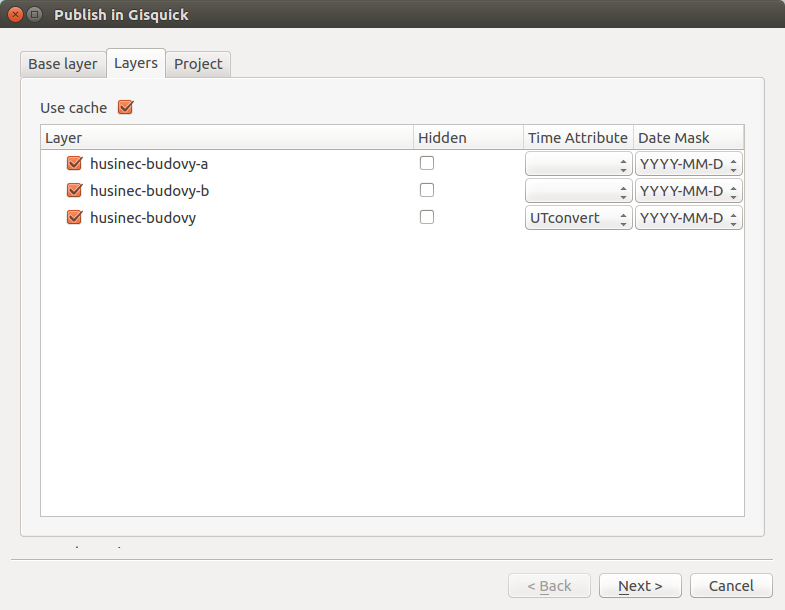
\includegraphics[width=0.75\textwidth]{../img/plugin-layers.png}
	\caption{Time layers options in publication wizard}
	\label{fig:publication-wizard-layers}
\end{figure}

Every user should know how the data looks like. 
\textbf{Date Mask} changes user interface of the time filtering tool. 
E.g. if 'HH:mm' mask is selected date picker will not be 
displayed in the client side, only time picker. 

Its recommended to use time date in format starting with 
year e.g. 'YYYY-MM-DD'. Otherwise, new attribute containing time 
values in UNIX time format has to be created during publication 
process.

The \textbf{configuration summary} wizard page displays all the parameters 
that were computed for each time layer. Note that if the 
\textbf{Time Attribute} field was left blank, parameters will not have any 
value.

\begin{figure}[h!]
	\centering
	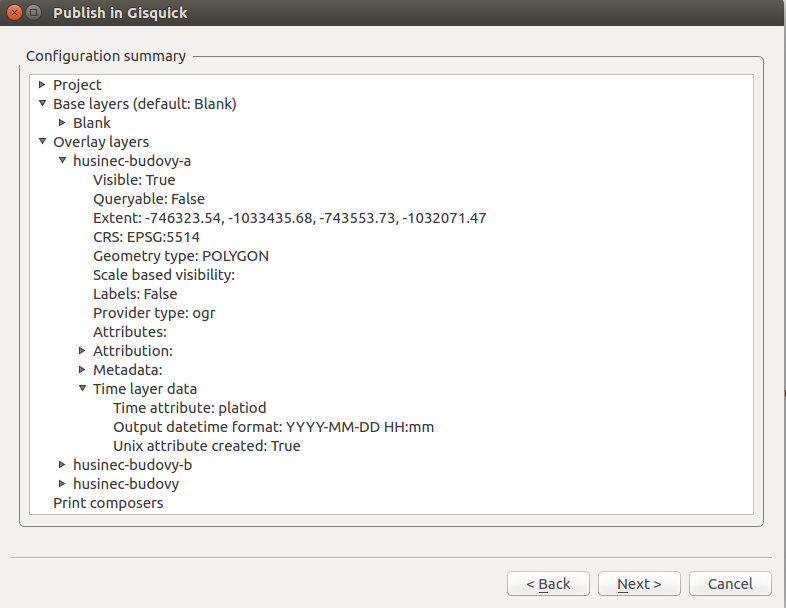
\includegraphics[width=0.7\textwidth]{../img/project-publishing-time-summary.png}
	\caption{Time layers publication summary}
	\label{fig:publication-wizard-summary}
\end{figure}

\bigskip
\noindent \textbf{Time filtering tool}

Time filtering tool in Gisquick client is available in the tool menu 
in upper left corner. 

\begin{figure}[h!]
	\centering
	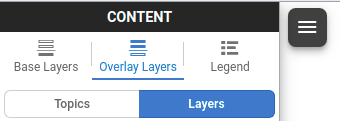
\includegraphics[width=0.4\textwidth]{../img/burger-menu.png}
	\caption{Tool menu}
	\label{fig:burger-menu}
\end{figure}

\bigskip
When the tool is activated dropdown menu with time layers appears on 
the left side of map canvas. For needs of filtration the time layer 
has to be specified. Despite selecting one time layer there is
also possibility of selecting \textit{All visible layers}.

\begin{figure}[h!]
	\centering
	
\includegraphics[width=0.4\textwidth]{../img/time-layers-dropdown.png}
	\caption{Dropdown menu containing time layers}
	\label{fig:time-layers-drpdown}
\end{figure}

\bigskip
It might happen that two time layers with different time extend are 
visible in the same time. E.g. one layer displaying map features 
over one hour and second over one year. Filtering this two layers 
together using one time slider would ignore layer with shorter time 
extend. That is the reason why only time layers with same time 
attribute may be displayed in the same time. In case `All visible 
layers` contains different time attribute. User have to specify one 
in displayed dropdown menu.

\begin{figure}[h!]
	\centering
	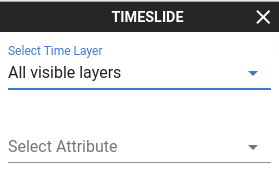
\includegraphics[width=0.4\textwidth]{../img/time-attribute-dropdown.png}
	\caption{Dropdown menu containing time attributes}
	\label{fig:time-attribute-dropdown}
\end{figure}

\newpage
Once filtering layer is specified various settings is displayed. 

\begin{figure}[h!]
	\centering
	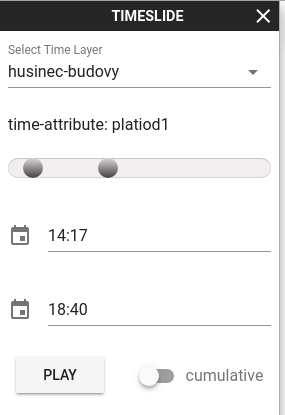
\includegraphics[width=0.4\textwidth]{../img/time-filtering-tool.png}
	\caption{Initialized time filtering tool}
	\label{fig:time-filtering-tool}
\end{figure}

Time filtering tool is composed of following parts:

\begin{itemize}
	\item\textit{Dropdown menu with time layers}
	\item\textit{Time attribute label}
	\item\textit{Double range slider}
	\item\textit{Lower and upper time value}
	\item\textit{Animation button with cumulative switch}
\end{itemize}

Function of \textbf{Dropdown menu with time layers} was mentioned before.
If selected time layer was already filtered, time filtering 
tool is initialized using previously used values.

\textbf{Time attribute label} displays name of attribute that was selected
in the process of project publishing as `Time Attribute`. This 
comes handy especially when `All visible layers` are selected.

\textbf{Double range slider} allows user to make fast data filtration.
Time interval is set using two sliders. Map content is refreshed 
each time the slider is changed. Step of double range slider is set 
as one hundredth of time interval size.

\begin{figure}[h!]
	\centering
	
\includegraphics[width=0.4\textwidth]{../img/time-slider.png}
	\caption{Double range slider}
	\label{fig:time-slider}
\end{figure}

Time interval may be specified with better precision than time 
slider using \textbf{Lower and upper time value} labels. Precision depends
on selected output time format in project publication. If format 
contains time and date, then labels allow user to set time using time
pickers and date in calendar. In case that time format contains date 
than is not more precise than one day, only calendar is displayed. 
Time and date 
selection in displayed date time picker has to be confirmed by 
\textit{OK} button. Map canvas is updated after this confirmation.

\begin{figure}[h!]
	\centering
	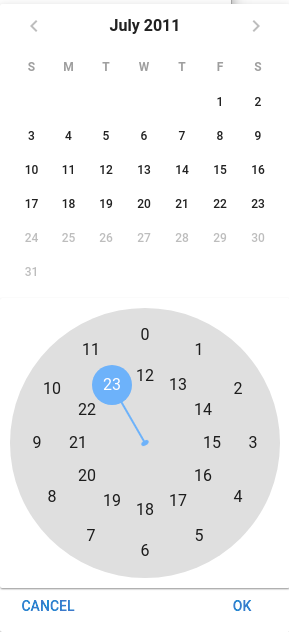
\includegraphics[width=0.3\textwidth]{../img/date-time-picker.png}
	\caption{Date time picker}
	\label{fig:date-time-picker}
\end{figure}

Simple animation can be made using \textbf{Animation button}. There are two 
options. Classic and cumulative animation. Classical one increases both 
upper and lower values every second by slider step. 
Animation stops when upper value reach slider maximum. If cumulative 
mode is turned on only upper value is being increased. When it reaches 
slider maximum than lower value increases in the same pattern.
Animation ends when difference between upper and lower value is just one 
step. Second  way how to stop animation may be click on \textit{STOP} button. 
Stop button appears only when animation is on. Map canvas is updated 
each time when slider value is changed.

\begin{figure}[h!]
	\centering
	
\includegraphics[width=0.4\textwidth]{../img/time-animation-stop.png}
	\caption{Time animation stop button}
	\label{fig:time-animation-stop}
\end{figure}

\newpage
\section{Seznam obrázků a tabulek}
\listoffigures
\listoftables




\end{document}
